\documentclass[natbib,preprint]{sigplanconf}

\usepackage[usenames]{color}
\definecolor{citationcolour}{rgb}{0,0.4,0.2}
\definecolor{linkcolour}{rgb}{0,0,0.8}
\usepackage{hyperref}
\hypersetup{colorlinks=true,
            urlcolor=linkcolour,
            linkcolor=linkcolour,
            citecolor=citationcolour,
            pdftitle=Relational Parametricity for Algebraically-Indexed Types,
            pdfauthor={Robert Atkey, Neil Ghani, Patricia Johann, Andrew Kennedy},
            pdfkeywords={}}  
\def\sectionautorefname{Section}
\def\subsectionautorefname{Section}
\def\subsubsectionautorefname{Section}

\title{Relational Parametricity for Algebraically Indexed Types}

\authorinfo{Robert Atkey\and Neil Ghani\\\and Patricia Johann}
           {University of Strathclyde}
           {\{Robert.Atkey,Neil.Ghani,Patricia.Johann\}@cis.strath.ac.uk}

\authorinfo{Andrew Kennedy}
           {Microsoft Research Cambridge}
           {akenn@microsoft.com}

\usepackage{mathpartir}
\usepackage{amsmath}
\usepackage{amssymb}
\usepackage{amsthm}
\usepackage{stmaryrd}
\usepackage[all]{xy}

\newcommand{\todo}[1]{[\textbf{TODO}: #1]}

\newcommand{\GL}[1]{\mathrm{GL}_#1}
\newcommand{\SynGL}[1]{\mathsf{GL}_#1}
\newcommand{\SynSE}[1]{\mathsf{SE}_#1}
\newcommand{\Orth}[1]{\mathrm{O}_#1}
\newcommand{\SynOrth}[1]{\mathsf{O}_#1}
\newcommand{\Transl}[1]{\mathrm{T}_#1}
\newcommand{\SynTransl}[1]{\mathsf{T}_#1}

% \newcommand{\GLtwo}{\mathrm{GL}_2}
% \newcommand{\SynGLtwo}{\mathsf{GL}_2}
% \newcommand{\GLone}{\mathrm{GL}_1}
% \newcommand{\SynGLone}{\mathsf{GL}_1}

\newcommand{\sepbar}{\mathrel|}

\newcommand{\Rel}{\mathrm{Rel}}
\newcommand{\relArrow}{\mathrel{\widehat\to}}
\newcommand{\relTimes}{\mathrel{\widehat\times}}
\newcommand{\relSum}{\mathrel{\widehat+}}

\newcommand{\setOfIntegers}{\mathbb{Z}}
\newcommand{\setOfBooleans}{\{\tmTT, \tmFF\}}

\newcommand{\id}{\mathrm{id}}

\newcommand{\SortSet}{\mathit{Sort}}
\newcommand{\IndexOpSet}{\mathit{IndexOp}}
\newcommand{\PrimTypeSet}{\mathit{PrimType}}
\newcommand{\IndexAxiomSet}{\mathit{IndexAx}}

\newcommand{\indexOp}[1]{\texttt{#1}}
\newcommand{\idxTms}[2]{\mathrm{IdxTm}(#1 \vdash #2)}
\newcommand{\idxTmAS}[1]{\mathrm{IdxTm}(#1)}

\newcommand{\tyInt}{\texttt{int}}
\newcommand{\tyBool}{\texttt{bool}}
\newcommand{\tyUnit}{\texttt{unit}}
\newcommand{\tyReal}{\texttt{real}}
\newcommand{\tyPrim}[2]{\textup{\texttt{#1}}\langle #2 \rangle}
\newcommand{\tyPrimNm}[1]{\texttt{#1}}
\newcommand{\primTyArity}{\mathrm{tyArity}}
\newcommand{\indexOpArity}{\mathrm{opArity}}

\newcommand{\tyArr}{\to}
\newcommand{\tyProduct}{\times}
\newcommand{\tyX}[1]{\texttt{X}\langle #1 \rangle}
\newcommand{\isType}{\textsf{ type}}
\newcommand{\isCtxt}{\textsf{ ctxt}}
\newcommand{\Ty}{\textsf{Ty}}
\newcommand{\ty}{\textsf{ty}}

\newcommand{\tmTT}{\texttt{tt}}
\newcommand{\tmFF}{\texttt{ff}}

\newcommand{\relEnv}[1]{\mathcal{#1}}
\newcommand{\tySem}[1]{\llbracket #1 \rrbracket^{\mathcal{T}}}
\newcommand{\ctxtSem}[1]{\llbracket #1 \rrbracket^{\mathcal{C}}}
\newcommand{\tmSem}[1]{\llbracket #1 \rrbracket^{\mathit{tm}}}
\newcommand{\tyPrimSem}[1]{\llbracket #1 \rrbracket^{\mathcal{T}_0}}
\newcommand{\rsem}[3]{\llbracket #1 \rrbracket^{\mathcal{R}}_{#2}{#3}}
\newcommand{\extends}[2]{\mathsf{ext}(#1,#2)}

\newtheorem{lemma}{Lemma}
\newtheorem{theorem}{Theorem}
\newcommand{\lemref}[1]{\hyperref[#1]{Lemma \ref*{#1}}}
\newcommand{\thmref}[1]{\hyperref[#1]{Theorem \ref*{#1}}}
\newcommand{\propref}[1]{\hyperref[#1]{Proposition \ref*{#1}}}
\newcommand{\corref}[1]{\hyperref[#1]{Corollary \ref*{#1}}}
\newcommand{\conref}[1]{\hyperref[#1]{Conjecture \ref*{#1}}}
\newcommand{\exref}[1]{\hyperref[#1]{Example \ref*{#1}}}
\newcommand{\statementref}[1]{\hyperref[#1]{Statement \ref*{#1}}}

\newcommand{\sem}[1]{\llbracket #1 \rrbracket}
\newcommand{\isDefinedAs}{\stackrel{\mathit{def}}=}

\newtheoremstyle{examplestyle}
  {\topsep}  % space above
  {\topsep}  % space below
  {\normalfont}% name of font to use in the body of the theorem
  {0em}% measure of space to indent
  {\bfseries}% name of head font
  {.}% punctuation between head and body
  {5pt plus 1pt minus 1pt}% space after theorem head; " " = normal interword space
  {}% Manually specify head
\theoremstyle{examplestyle}
\newtheorem{example}{Example}

\newtheoremstyle{restatementstyle}
  {\topsep}  % space above
  {\topsep}  % space below
  {\itshape}% name of font to use in the body of the theorem
  {0em}% measure of space to indent
  {\bfseries}% name of head font
  {.}% punctuation between head and body
  {5pt plus 1pt minus 1pt}% space after theorem head; " " = normal interword space
  {\thmname{#1} \thmnote{(Restatement of #3)}}% Manually specify head
\theoremstyle{restatementstyle}
\newtheorem{restateLemma}{Lemma}
\newtheorem{restateTheorem}{Theorem}

\newcommand{\fixme}[1]{\textbf{FIXME: #1}}

\begin{document}

\maketitle

\begin{abstract}
  
\end{abstract}

\category{D.1.1}{Programming techniques}{Applicative (functional)
  programming} \category{D.2.4}{Software Engineering}{Software/Program
  Verification} \category{D.3.3}{Programming Languages}{Language
  Constructs and Features---Data types and structures}

\terms
  Languages, Theory, Types

\keywords
  parametricity, units of measure, dimensional analysis, invariance, computational geometry

%%%%%%%%%%%%%%%%%%%%%%%%%%%%%%%%%%%%%%%%%%%%%%%%%%%%%%%%%%%%%%%%%%%%%%%%%%%%%%
%%%%%%%%%%%%%%%%%%%%%%%%%%%%%%%%%%%%%%%%%%%%%%%%%%%%%%%%%%%%%%%%%%%%%%%%%%%%%%
\section{Introduction}
\label{sec:introduction}
The best way we know of describing the semantics of parametric
polymorphism is \emph{relational parametricity}, whose central result
is Reynolds' Abstraction Theorem~\cite{reynolds83types}. Its striking
consequences include the well-known ``free theorems'' for polymorphic
types~\cite{wadler89theorems}, non-inhabitation results, and precise
correspondences between System F encodings and algebraic
datatypes~\cite{PittsAM:parpoe}, abstract data types, and, most
recently, higher-order encodings of binder
syntax~\cite{syntaxforfree}.

Relational parametricity is in essence a principle of
\emph{invariance}: the behaviour of polymorphic code is invariant
under changes of data representation. For example, the type
$\forall\alpha.\tyPrim{list}\alpha\to\tyPrim{list}\alpha$
tells us that any transformation applied to elements of
the input list will be reflected by the same transformation applied
to elements of the result. 
Invariance results also abound in
mathematics and physics. The area of a triangle is invariant with
respect to isometries of the Euclidean plane; the determinant of a
matrix is invariant under changes of basis; and Newton's laws are the
same in all inertial frames. Typically, the 
transformations under which invariants are preserved have interesting structure: 
for example, translations in
the Euclidean plane form an abelian group.

Inspired by this connection, we study type systems that
capture rich invariants through types indexed by attributes with
algebraic structure.  For example, in computational geometry, points
in the plane can be indexed by attributes representing affine
transformations; in information-flow security, computations can be
indexed by principals; in differential privacy, types can be indexed
by `distance'. Types that are polymorphic over such indices induce
invariance properties and abstraction barriers beyond those introduced
by their unindexed versions, as we shall illustrate.  This generalises
previous work by the third author on types parameterized by
units of measure, whose invariance properties relate to changes of
units, or \emph{scaling}~\cite{kennedy97relational}.

Our motivations for studying algebraically indexed types are
threefold. First, we believe that, as with
units of measure~\cite{fsharp}, practical programming language
extensions will follow. For example, in computational geometry and
graphics, attributes on points, vectors, and other geometric types
could be used to prevent the mixing of different coordinate systems,
or `frames'. Second, type-based static analyses can be based on
indexed types, for example, in effect systems~\cite{benton06reading},
and, more speculatively, in continuity
analysis~\cite{chaudhuri10continuity}.  Finally, we believe that
expressing algebraic invariants through types has the potential to
offer slick proof techniques for mechanized
mathematics. Harrison has applied the
invariance properties of geometric primitives to create elegant proofs
in geometry, based on `without loss of
generality' principles~\cite{harrison09without}. The invariance properties are expressed 
and propagated using ad-hoc tactics; our types offer a more principled
means of achieving the same end, and the `wlog' principle itself
is expressed through type isomorphisms.

We follow the mantra \emph{semantics first, syntax later} in studying
types with algebraic structure. We have not yet built a practical
programming language that supports algebraically indexed types; nor
have we designed type checking, type inference, or static analysis
algorithms.  But when we do so, the semantics will guide us. The fact
that zero is polymorphic in units of measure (it can be given type $\forall
u.\tyPrim{real}u$) whereas other constants are dimensionless (having
type $\tyPrim{real}1$) is justified by the invariance properties
induced by the types: zero is invariant under scaling, other constants
are not. For less trivial constants and operations, the appropriate types are
not so apparent, as we shall see, but invariance properties expressed by
the semantics guide us in assigning appropriate types. Semantics does not lie!


\paragraph{Invariance}
To illustrate type-induced invariance properties, consider
2-dimensional geometry. 
A function $\mathit{areaTri}$ that computes the area of a triangle
can be assigned the type:
$\tyPrimNm{vec}\times\tyPrimNm{vec}\times\tyPrimNm{vec}\tyArr\tyReal$.
But we can also assign it the following more expressive polymorphic
type:
\[
\mathrm{areaTri} : \forall t\mathord:\SynTransl{2}.
  \tyPrim{vec}{t} \times \tyPrim{vec}{t} \times \tyPrim{vec}{t} \to \tyReal \\
\]
This type expresses the fact that if each of the arguments to $\mathrm{areaTri}$
is translated by the same vector, then the result remains the same,
that is, it is \emph{invariant} under translation. Formally, for any 
vector $\vec t$,
\[
\mathrm{areaTri}\;(\vec{t} + \vec{v_1}, \vec{t} + \vec{v_2}, \vec{t} + \vec{v_3}) = 
\mathrm{areaTri}\;(\vec{v_1}, \vec{v_2}, \vec{v_3})
\]

Transformations typically \emph{compose} in various
ways, and the compositions satisfy algebraic laws. For example, 
we can assign a function that computes the area of a circle given its
radius the following polymorphic type:
\[
\mathrm{areaCircle} : \forall s\mathord:\SynGL{1}.\tyPrim{real}{s}\to
\tyPrim{real}{s\cdot s}
\]
This captures the fact that the area of a circle varies as the square
of its radius, i.e., $\mathrm{areaCircle}(k r) = k^2\cdot
\mathrm{areaCircle}(r)$ for any $k\neq 0$ (the `sorts' $\SynTransl{2}$ and
$\SynGL{1}$ will be explained later).  Here, $s$ 
can be interpreted as the \emph{units of measure} of the argument to
$\mathrm{areaCircle}$, and `$\cdot$' composes units using the
product. We can also add an inverse operation and identity unit of
measure $1$, and then impose the algebraic laws of abelian
groups. This permits identification of, for example,
$\tyPrim{real}{s\cdot s^{-1}}$ with the type
$\tyPrim{real}{1}$ of dimensionless constants.

\paragraph{Abstraction}
In his original paper on parametricity, Reynolds asserted that
\emph{type structure is a syntactic discipline for enforcing levels of
  abstraction}.  We see something analogous here: if all primitive
operations are given types that reflect their behaviour under
translation, then there is no way to `break' this property. For
example, there is no way that $\mathrm{areaTri}$ can depend on the
actual coordinates of its inputs. Furthermore, the distinction between
points and vectors that is often enforced through abstract data
types~\cite{CGAL} is captured here by indices instead. For example,
the operation that takes two points and computes their vector
difference can be assigned the type
$\forall t\mathord:\SynTransl{2}.\tyPrim{vec}t\times\tyPrim{vec}t\to\tyPrim{vec}0$,
reflecting the invariance of the result (a pure vector) under
translations of the point arguments. As a result through types alone
we can, in essence, derive so-called \emph{coordinate-free}
geometry~\cite{CFGADT}.

The invariance properties discussed above can be seen as ``free
theorems''~\cite{wadler89theorems}, but the abstraction afforded by
polymorphic indexed types can also induce interesting type
\emph{isomorphisms}.  The type of $\mathrm{areaCircle}$ above is in
fact isomorphic to $\tyPrim{real}{1}$. A moment's thought reveals why:
what possible unary functions can be constructed whose outputs scale
as the square of the scaling of their inputs?  Answer: just those
functions of the form~$\lambda x. k x^2$ for some constant~$k$.  In
this case, of course, we expect that~$k = \pi$.

\paragraph{Relational parametricity}
To derive such invariance and abstraction properties of types, we
adopt the techniques of relational parametricity. Over an underlying
index-erasure semantics we construct binary relations parameterised by
an environment $\rho$ that describes how values of primitive type are
related according to their indices.  For example, values $v$ and $w$
of type $\tyPrim{real}s$ are related when $v$ ``scales to'' $w$
according to an interpretation of $s$ (i.e., $w=\rho(s)\cdot
v$).  Values of polymorphic type are related exactly when they are
related for all possible interpretations of the quantified
variable. For example, values $v$ and $w$ of type
$\forall t\mathord:\SynTransl{2}.\tyPrim{vec} t\to
\tyPrim{vec} t$ are related when they are related at type
$\tyPrim{vec} t\to\tyPrim{vec}t$ for all translations
$\vec t\in\Transl{2}$ associated with $t$.

As it happens, the relational interpretations given above are
functional, relating one value uniquely to another. Other applications
make use of primitive relations that are not simple functions.
For example, in a type system in which the index in
$\tyPrim{real}s$ is interpreted not as a unit of measure, but as
a measure of \emph{closeness}, two values $x$ and $y$ of this type are
related if $|x-y| < \rho(s)$ for a positive real number
$\rho(s)$.  Rather beautifully, the standard notion of uniform
continuity can then be expressed as %a type:
%\begin{displaymath}
 $ \forall \epsilon \mathord: \mathsf{R}^{>0}.\ \exists \delta\mathord: \mathsf{R}^{>0}.\ \tyPrim{real}{\delta} \to \tyPrim{real}{\epsilon}$.
%\end{displaymath}


% Possible angles of attack:
% \begin{itemize}
% \item Parametric polymorphic types allow us to prevent
%   over-specification of the behaviour of programs. For instance, the
%   type $\forall \alpha. [\alpha] \to [\alpha]$ is a generalisation of
%   the types $[\mathsf{int}] \to [\mathsf{int}]$ and $[\mathsf{char}]
%   \to [\mathsf{char}]$. Either of the latter two types over-specify
%   the behaviour of the function.
% \item There are other cases of programs that are over-specified. The
%   leading example we just below is of geometric programs that
%   manipulate coordinate data. Often, programs that manipulate
%   coordinate data are insensitive to geometric transformations. For
%   example, a program that computes the area of a triangle described by
%   three points is insensitive to translations or rotations applied to
%   all three points.
% \item 
% \end{itemize}

% There are three main points to get across:
% \begin{enumerate}
% \item Why algebraically indexed types?
% \item Why relational parametricity?
% \item Why study them together?
% \end{enumerate}

\subsection{Contributions}
\label{sec:contributions}

\begin{figure}
  \centering
  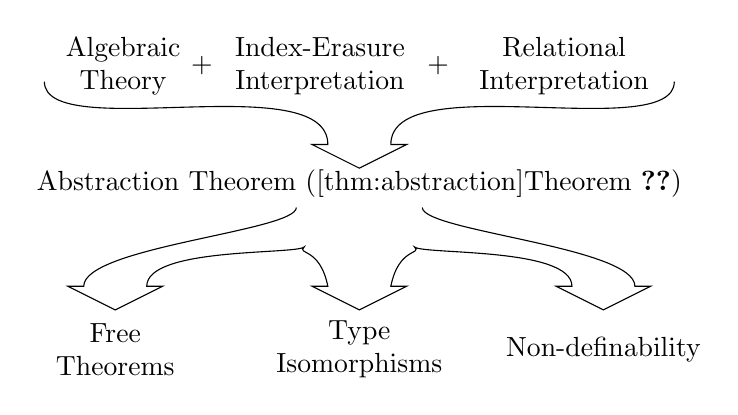
\begin{tikzpicture}
  \node at (-3,0.8) [rectangle,style={align=center}] {Algebraic \\ Theory};
  \node at (-2,0.8) {$+$};
  \node at (-0.5,0.8) [rectangle,style={align=center}] {Index-Erasure \\ Interpretation};
  \node at (1,0.8) {$+$};
  \node at (2.6,0.8) [rectangle,style={align=center}] {Relational \\ Interpretation};
  
  \draw plot (-4,0.6) .. controls (-4,-0.2) and (-0.4,0.8) .. (-0.4,-0.2)
             -- (-0.6,-0.2) -- (0,-0.5) -- (0.6,-0.2) --
             (0.4,-0.2) .. controls (0.4,0.8) and (4,-0.2) .. (4,0.6);

  \node at (0,-0.7) [rectangle,style={align=center}] {Abstraction Theorem (\thmref{thm:abstraction})};

  \draw plot (-0.8,-1) .. controls (-0.8,-1.3) and (-3.5,-1.5) .. (-3.5,-2)
             -- (-3.7,-2) -- (-3.1,-2.3) -- (-2.5,-2) -- 
             (-2.7,-2) .. controls (-2.7,-1.5) and (-0.8,-1.6) .. (-0.7,-1.5)
                       .. controls (-0.8,-1.6) and (-0.5,-1.5) ..
             (-0.4,-2) -- (-0.6,-2) -- (0,-2.3) -- (0.6,-2) --
             (0.4,-2) .. controls (0.5,-1.5) and (0.8,-1.6) .. (0.7,-1.5)
                      .. controls (0.8,-1.6) and (2.7,-1.5) ..
             (2.7,-2) -- (2.5,-2) -- (3.1,-2.3) -- (3.7,-2) -- (3.5,-2)
                      .. controls (3.5,-1.5) and (0.8,-1.3) .. (0.8,-1);

  \node at (-3.1,-2.8) [rectangle,style={align=center}] {Free \\ Theorems};
  \node at (0,-2.8) [rectangle,style={align=center}] {Type \\ Isomorphisms};
  \node at (3.1,-2.8) [rectangle,style={align=center}] {Non-definability};
\end{tikzpicture}
  \caption{Summary of the Paper}
  \label{fig:summary}
\end{figure}

This paper makes the following specific contributions:
\begin{itemize}
\item 
We present a collection of compelling examples of algebraically
indexed types, including a novel type system for geometry, a
refined type system for information flow based on logic, and a simple
type system with distance-indexed types.
\item 
We formulate a type system that can either be used as a programming
language in its own right, or as the target of type-based
analyses. The type system consists of the usual type constructors
together with a collection of indexed primitive types, universal and
existential quantification over the indices, and a multi-sorted
equational theory for indices.
\item
We describe a relational semantics for the type system and prove an
analogue of Reynolds' Abstraction Theorem, for a given \emph{model}
of index sorts and relational interpretation of primitive types.
We prove that the semantics soundly approximates contextual equivalence.
\item
For each of our main examples we deduce free theorems that are
consequences of our Abstraction Theorem, prove non-definability
results, and derive interesting type isomorphisms. \autoref{fig:summary}
illustrates the central position of our analogue of Reynolds' Abstraction
Theorem (\thmref{thm:abstraction}) in these results.
\item
We improve on the earlier semantics of
units of measure~\cite{kennedy97relational} in a number of ways.  By
extending the language of units with an `absolute value' operation, we
can give more precise types and obtain more general invariance
properties.  The relational interpretation for units is both simpler
and more flexible, and we derive slicker proofs of non-definability,
and new results.  Our notion of type isomorphism is stronger than
previously, being based on contextual equivalence.
\end{itemize}
We have fully formalised our framework and most examples in Coq,
using strongly-typed term representations
throughout~\cite{TypedSyntax}. The formalisation is available from
\\{\small \url{https://github.com/bobatkey/algebraically-indexed-types}}



%%% Local Variables:
%%% TeX-master: "paper"
%%% End:

\section{Motivating Examples}
\label{sec:motivating-examples}

We motivate this paper's goal of investigating algebraically-indexed
types and their relational interpretations by presenting several
examples. Our leading example is a novel type system for writing
programs that manipulate geometric data, while maintaining geometric
invariants through the types. The other examples are enforcement of
information flow properties via indexing by a logical theory
(\autoref{sec:information-flow}), and incorporation of metric
properties into types (\autoref{sec:continuity-analysis}).

\subsection{2-Dimensional Geometry and Origin Invariance}

When writing programs that manipulate geometric data, the basic data
structure is the $n$-tuple of numbers. In the 2-dimensional case,
tuples $\vec{v} = (x,y)$ are called upon to represent both
\emph{points}---offsets from some origin---and
\emph{vectors}---offsets in their own right. Points and vectors are
very different despite their common representation.

Distinguishing between points and vectors is the key feature of
\emph{affine geometry} (see, for example, Gallier's book
\cite{gallier11geometric}, Chapter 2). Traditionally in computational
geometry libraries, the distinction between points and vectors has
either been left to the programmer to maintain by themselves, or has
been enforced through the use of separate abstract types for points
and vectors (one might say that the standard mathematical formulation
of affine spaces uses the abstract types approach). Here, we
investigate a more sophisticated approach using types indexed by
change of origin transformations, and think of the difference between
points and vectors as a change of data representation.

Putting this in concrete terms, if we have two origins, $(0,0)$ and
$(10,20)$, then the tuple $(1,1)$ with respect to the first origin and
$(11,21)$ with respect to the second origin represent the \emph{same}
point. It is merely an artifact of our representation of points as
pairs of numbers that these appear to be different. When we write
programs that manipulate data that represents points, we ought to
ensure that our programs are invariant with respect to changes in the
choice of origin. On the other hand, vectors are not intended to be
regarded as invariant under change of origin. Vectors represent
offsets, or movements, and the vector $(0,0)$ always represents the
zero offset.

Invariance under change of representation immediately recalls
Reynolds' fable concerning two professors teaching the theory of
complex numbers \cite{reynolds83types}. One professor chooses
rectangular coordinates ($x + iy$), while the other chooses polar
coordinates ($\alpha\cos\theta + i\alpha\sin\theta$). Happily, after
learning the basic operations on complex numbers in the two
representations, the two classes can interact because the theory of
complex numbers is invariant with respect to the choice of
representation. Reynolds formalises the idea of invariance with
respect to changes of representation as preservation of relations. If
a binary relation $R$ relates two representations of a concept---for
example the rectangular and polar representations of the same complex
number are related---then a program that manipulates complex numbers
at a level of abstraction above their specific representation should
preserve the relation $R$. For example, let $f$ be a program taking
complex numbers to complex numbers that is intended to respect
invariance under change of representation. Then if $c$ is a complex
number in rectangular form, and $c'$ is a complex number in polar form
such that $R$ relates them, which we write as $(c,c') \in R$, then it
should be the case that $(f(c), f(c')) \in R$.

We now apply Reynolds' relational approach to the geometric
setting. We define a family of binary relations on $\mathbb{R}^2$
which is indexed by changes of origin. Changes of origin are
represented by vectors in $\mathbb{R}^2$, and form a group under
addition. To emphasise the group structure, and the intended meaning
as translations, we write the collection of all change of origin
offsets as $\Transl_2$. By quantifying over all changes of origin we
will be able to ensure that our programs are invariant with respect to
the particular choice of origin. The members of the
$\Transl_2$-indexed family of binary relations $\{ R_{\vec{t}}
\subseteq \mathbb{R}^2 \times \mathbb{R}^2 \}_{\vec{t} \in \Transl_2}$
are defined as follows:
\begin{displaymath}
  R_{\vec{t}} = \{ (\vec{v}, \vec{v'}) \sepbar \vec{v'} = \vec{v} + \vec{t} \}
\end{displaymath}

Now consider a function $f$ that, for example, takes two tuples in
$\mathbb{R}^2$ and returns a single tuple in $\mathbb{R}^2$. We intend
that all these tuples represent points with respect to the same
origin, but that the function itself should be invariant with respect
to the choice of origin. We use Reynolds' idea of preservation of
relations to formalise this: for any $\vec{t} \in \Transl_2$ (i.e.~any
change of origin), the function $f$ should satisfy the following
statement:
\begin{equation}\label{eq:f-preserve-rel-frame}
  \forall (\vec{v_1},\vec{v'_1}) \in R_{\vec{t}}, (\vec{v_2},\vec{v'_2}) \in R_{\vec{t}}. (f(\vec{v_1}, \vec{v_2}), f(\vec{v'_1}, \vec{v'_2})) \in R_{\vec{t}}
\end{equation}
Unfolding the definition of $R_{\vec{t}}$, this statement is
equivalent to the following statement expressing invariance of $f$
with respect to changes of origin: for all $\vec{t} \in \Transl_2$:
\begin{equation}\label{eq:f-invariant-frame}
  \forall \vec{v_1}, \vec{v_2}.\ f(\vec{v_1} + \vec{t},\vec{v_2} + \vec{t}) = f(\vec{v_1},\vec{v_2}) + \vec{t}.
\end{equation}
So Reynolds' preservation of relations, when instantiated with the
family of relations $\{R_{\vec{t}}\}$, yields exactly the geometric
property of invariance under change of origin.

% An example function $f$ that satisfies
% \statementref{eq:f-invariant-frame} is the following function that
% computes a particular affine combination of two points by working
% directly on their coordinate representation:
% \begin{displaymath}
%   f(\vec{v_1}, \vec{v_2}) = \frac{1}{2}\vec{v_1} + \frac{1}{2}\vec{v_2}.
% \end{displaymath}
% In general, affine combinations of points $\lambda_1\vec{v_1} +
% \lambda_2\vec{v_2}$, where $\lambda_1 + \lambda_2 = 1$, satisfy
% \statementref{eq:f-invariant-frame}. Affine combination is one of the
% fundamental building blocks of affine geometry -- the properties of
% points invariant under invertible affine maps
% (\cite{gallier11geometric}, Chapter 2). If we drop the condition that
% $\lambda_1 + \lambda_2 = 1$, then we are dealing with linear
% combinations of vectors, and we are no longer invariant with respect
% to changes of frame. However, linear combinations are invariant with
% respect to change of basis. We can represent changes of basis as
% linear invertible maps $B : \mathbb{R}^2 \to \mathbb{R}^2$. The set of
% all such maps forms the general linear group $\GL(2)$. We now define
% another family of relations $\{R_{\texttt{vec}}(B) \subseteq
% \mathbb{R}^2 \times \mathbb{R}^2 \}_{B \in \GL(2)}$ that relates two
% points up to change of basis:
% \begin{displaymath}
%   R_{\texttt{vec}}(B) = \{ (\vec{v_1},\vec{v_2}) \sepbar B\vec{v_2} = \vec{v_1} \}.
% \end{displaymath}
% Now the functions $f_{\lambda_1\lambda_2}(\vec{v_1},\vec{v_2}) =
% \lambda_1\vec{v_1} + \lambda_2\vec{v_2}$, for arbitrary $\lambda_1$
% and $\lambda_2$, do preserve the relations $R_{\texttt{vec}}(B)$, for
% all $B \in \GL(2)$. Unfolding the definition of $R_{\texttt{vec}}(B)$
% in the analogous statement to \statementref{eq:f-preserve-rel-frame}
% for $R_{\texttt{vec}}$ instead of $R_{\texttt{pt}}$, we can see that
% preservation of the relations $R_{\texttt{vec}}$ characterises the
% functions that are invariant under change of basis. For all $B \in \GL(2)$, we have
% \begin{displaymath}
%   \forall \vec{v_1}, \vec{v_2}.\ f(B\vec{v_1},B\vec{v_2}) = B(f(\vec{v_1},\vec{v_2})),
% \end{displaymath}
% and this is exactly the property of invariance under change of basis
% we required above of programs manipulating vectors.

% Note that the family of relations $R_{\texttt{vec}}$ is just
% $R_{\texttt{pt}}$ when restricted to elements of the group
% $\GL(2)$. In the type system we introduce in the next section, we
% combine points and vectors into the same data type. Whether it
% represents a point or a vector depends on the group of geometric
% transformations that we expect it to be invariant under.

% FIXME: vectors are not invariant under change of origin, so they are
% represented by the relation $R_0$, which is just equality. But they,
% and points are invariant under change of basis. However, as we shall
% see below, not all operations are invariant under all changes of
% basis. In particular the dot product is only invariant under
% orthogonal transformations.

\subsection{A Type System for Origin Invariance}
\label{sec:type-system-geom-intro}

Reynolds' further insight was to see how preservation of relations by
the denotational interpretations of programs can automatically be
established by following a typing discipline. In Reynolds' case, the
typing discipline was the polymorphic $\lambda$-calculus where new
types can be constructed by universal quantification over all
types. Universal type quantification is commonly written $\forall
\alpha. A$, which denotes a type that may be instantiated with any
other type $B$ by replacing the type variable $\alpha$ with $B$ in
$A$.

In terms of relations, Reynolds interprets universal quantification
over types as quantification over binary relations between denotations
of types. In the statements of geometric invariance that we stated in
the previous section (e.g., \statementref{eq:f-invariant-frame}), we
did not quantify over all relations. Instead, we quantified over all
changes of origin and used the choice to select a relation from the
family $\{R_{\vec{t}}\}$. Driven by this observation, we introduce
quantification over changes of origin into the language of types.  We
use the notation $\forall t \mathord: \SynTransl_2. A$ for
quantification over all 2-dimensional translations (i.e.~choices of
origin) $t$. We refer to $\SynTransl_2$ as the \emph{sort} of
$t$. Note that we have used a different font to distinguish the
semantic group $\Transl_2$ from the syntactic sort $\SynTransl_2$.

The sort $\SynTransl_2$ represents an abelian group, so we can combine
its elements using the usual group operations. We write operations
additively, using $e_1 + e_2$ for the group operation, $-e$ for
inverse and $0$ for the unit.  We also regard expressions built from
variables and the group operations up to the abelian group axioms. For
example, $e_1 + (e_2 + e_3)$ and $(e_1 + e_2) + e_3$ are to be
regarded as equivalent.

Our language of types also includes the common type constructors for
function types, $A \to B$, sum types $A + B$, unit type
$\tyPrimNm{unit}$ and tuple types $A \times B$. We also assume a
primitive type $\tyPrimNm{real}$, used to represent scalars. As we
noted at the start of the previous section, the central data structure
in geometric applications is the tuple of real numbers for
representing points and vectors. However, we cannot simply express
this as the type $\tyPrimNm{real} \times \tyPrimNm{real}$ because it
will not have the correct relational interpretation. (Two elements of
type $\tyPrimNm{real}$ will be related if and only if they are equal,
and hence two elements of $\tyPrimNm{real} \times \tyPrimNm{real}$
will be related if and only if they are equal, by Reynolds' definition
of the relational interpretation of tuple types.) Therefore, we
introduce a new type parameterised by expressions $e$ of sort
$\SynTransl_2$ to represent points \emph{and} vectors:
$\tyPrim{vec}{e}$. We have used the name $\tyPrimNm{vec}$, even though
we have taken pains to separate geometric points and vectors, to
recall the computer science notion of vector as a sequence of values
of homogeneous type which has a known length (in this case two).

We now sketch the interpretation of the types $\tyPrim{vec}{e}$ and
$\forall t\mathord:\SynTransl_2.A$. In our calculus, each type has two
interpretations: an index-erasure interpretation that ignores the
indexing expression $e$, and a relational interpretation as a binary
relation on the index-erasure interpretation. For now, we assume we
are given some way of turning an expression $e$ of sort $\SynTransl_2$
into an actual element $\sem{e}\rho$ of the group $\Transl_2$, under
some environment $\rho$ which tells how to interpret the free
variables. The (simplified) index-erasure and relation interpretations
of the types $\tyPrim{vec}{e}$ are:
\begin{displaymath}
  \begin{array}{l@{\hspace{0.5em}=\hspace{0.5em}}l}
    \tySem{\tyPrim{vec}{e}} & \mathbb{R}^2 \\
    \rsem{\tyPrim{vec}{e}}{}\rho & R_{\sem{e}\rho} = \{ (\vec{v},\vec{v'}) \sepbar \vec{v'} = \vec{v} + \sem{e}\rho \}
  \end{array}
\end{displaymath}
The index-erasure interpetation of universal quantification $\forall
t\mathord:\SynTransl_2.A$ is simply the interpretation of the
underlying type $A$. The relational interpretation intersects the
relational interpretations of the type $A$ under all extensions of the
relational environment $\rho$:
\begin{displaymath}
  \begin{array}{l@{\hspace{0.5em}=\hspace{0.5em}}l}
    \tySem{\forall t\mathord:\SynTransl_2.A} & \tySem{A} \\
    \rsem{\forall t\mathord:\SynTransl_2.A}{}\rho & \bigcap\{ \rsem{A}{}{\rho'} \sepbar \rho' \in \extends{\rho}{t\mathord:\SynTransl_2} \}
  \end{array}
\end{displaymath}
The exact definition of $\extends{\rho}{t\mathord:\SynTransl_2}$
depends on which (possibly non-compositional) interpretation of
relational environments that we take. For now, it will suffice to
think of relational environments as simply mappings from free
variables of sort $\SynTransl_2$ to the group $\Transl_2$, and
extension as just adding an extra component to the tuple. The general
index-erasure semantics will be given in
\autoref{sec:index-erasure-semantics}. The relational interpretation
is in general more complex, due to the possibility of
non-compositional interpretations of free index variables. The
relational interpretation will be presented in
\autoref{sec:relational-semantics}.

In the previous section, we discussed functions $f : \mathbb{R}^2
\times \mathbb{R}^2 \to \mathbb{R}^2$ that have the property that they
preserve all changes of origin. We can now express this property as a
type:
\begin{displaymath}
  \mathrm{f} : \forall t \mathord: \SynTransl_2.\ \tyPrim{vec}{t} \times \tyPrim{vec}{t} \to \tyPrim{vec}{t}
\end{displaymath}
Spelling out the relational interpretation of this type using the
definitions above (and the standard relational interpretations for
tuple and function types), we obtain
\statementref{eq:f-invariant-frame}.

\subsection{Affine and Vector Operations}
\label{sec:affine-vector-ops}

Invariance under change of origin is the key feature of affine
geometry, and the central operation of affine geometry is the affine
combination of points: $\lambda_1\vec{v_1} + \lambda_2\vec{v_2}$,
where $\lambda_1 + \lambda_2 = 1$. Geometrically, affine combination
can be interpreted as interpolation between the points represented by
$\vec{v_1}$ and $\vec{v_2}$. We add affine combination of points to
our calculus, with the following typing and intended denotation:
\begin{displaymath}
  \begin{array}{l}
    \mathrm{affComb} :\forall t \mathord: \SynTransl_2.\ \tyPrim{vec}{t} \to \tyPrimNm{real} \to \tyPrim{vec}{t} \to \tyPrim{vec}{t} \\
    \sem{\mathrm{affComb}}\ \vec{v_1}\ r\ \vec{v_2} = (1-r)\vec{v_1} + r\vec{v_2}
  \end{array}
\end{displaymath}
It can be verified by hand that the intended denotation
$\sem{\mathrm{affComb}}$ has the invariance property specified by its
type.
% By defining the primitive function $\mathrm{affComb}$ to take a
% single $\tyPrimNm{real}$ parameter $t$, we can easily ensure that we
% are taking the affine combination of two representatives of points,
% and not just an arbitrary linear combination.

\begin{example}
  The evaluation of quadratic B\'{e}zier curves (B\'{e}zier curves
  with two endpoints and a single control point) can be expressed
  using the affine combination primitive and three steps of De
  Casteljau's algorithm:
  \begin{displaymath}
    \begin{array}{@{}l}
      \mathrm{quadB\acute{e}zier} : \forall t \mathord:\SynTransl_2.\ \tyPrim{vec}{t} \to \tyPrim{vec}{t} \to \tyPrim{vec}{t} \to \tyPrimNm{real} \to \tyPrim{vec}{t} \\
      \mathrm{quadB\acute{e}zier}\ [t]\ p_0\ p_1\ p_2\ s = \\
      \quad \mathrm{affComb}\ [t]\ (\mathrm{affComb}\ [t]\ p_0\ s\ p_1)\ s\ (\mathrm{affComb}\ [t]\ p_1\ s\ p_2) \\
    \end{array}
  \end{displaymath}
  For two endpoints $p_0$ and $p_2$ and a control point $p_1$, an
  application $\mathrm{quadB\acute{e}zier}\ p_0\ p_1\ p_2\ s$ for $s
  \in [0,1]$ gives us the point on the curve at ``time'' $s$. Note
  that the type of $\mathrm{quadB\acute{e}zier}$ tells us immediately
  that it preserves all changes of origin.
\end{example}

% Affine combination only provides us with an operation on points. We
% are also interested in operations on the vectors representing offsets
% between points. We now examine the correct types to assign to the
% vector space operations of addition of vectors, negation of vectors,
% multiplication by a scalar and the zero vector. The typings of these
% operations will make use of the abelian group structure of change of
% origin translations.

Vector operations are not invariant under change of origin. The
obvious type for vector addition is therefore:
\begin{displaymath}
  (+) : \tyPrim{vec}{0} \to \tyPrim{vec}{0} \to \tyPrim{vec}{0}
\end{displaymath}
(we write binary operators intended to be used infix in parentheses
when not appearing in infix position, following the Haskell
syntax.)

However, it is possible to give vector addition a more precise type
that shows how it is variant with change of origin:
\begin{displaymath}
  (+) : \forall t_1, t_2 \mathord: \SynTransl_2.\ \tyPrim{vec}{t_1} \to \tyPrim{vec}{t_2} \to \tyPrim{vec}{t_1 + t_2}
\end{displaymath}
We can also negate vectors, yielding a vector which points in the
opposite direction. Negation negates translation arguments:
\begin{displaymath}
  \mathrm{negate} : \forall t \mathord: \SynTransl_2.\ \tyPrim{vec}{t} \to \tyPrim{vec}{-t}
\end{displaymath}
With the primitive operations of addition and negation of vectors, we
can define the derived operation of subtraction:
\begin{displaymath}
  \begin{array}{l}
    (-) : \forall t_1,t_2 \mathord:\SynTransl_2.\ \tyPrim{vec}{t_1} \to \tyPrim{vec}{t_2} \to \tyPrim{vec}{t_1 - t_2} \\
    (-)\ [t_1]\ [t_2]\ p_1\ p_2 = p_1 + \mathrm{negate}\ p_2
  \end{array}
\end{displaymath}

Given two points that have been constrained to be invariant with
respect to the same change of origin---i.e.~two values of type
$\tyPrim{vec}{t}$---we can compute their offset, which is a vector
expressed with respect to the null change of origin. The offset
operation is a special case of vector subtraction:
\begin{displaymath}
  \begin{array}{l}
    \mathrm{offset} : \forall t \mathord:\SynTransl_2.\ \tyPrim{vec}{t} \to \tyPrim{vec}{t} \to \tyPrim{vec}{0} \\
    \mathrm{offset}\ [t]\ p_1\ p_2 = p_1 - p_2
  \end{array}
\end{displaymath}
Note how the type of the result of $\mathrm{offset}$ simplifies from
$\tyPrim{vec}{t-t}$ to $\tyPrim{vec}{0}$. The algebraic structure on
the indexing theory induces type equalities.  The type of the vector
addition operation can be specialised to the case of moving a point by
a vector:
\begin{displaymath}
  \begin{array}{l}
    \mathrm{moveBy} : \forall t \mathord:\SynTransl_2.\ \tyPrim{vec}{t} \to \tyPrim{vec}{0} \to \tyPrim{vec}{t} \\
    \mathrm{moveBy}\ [t]\ p\ v = p + v
  \end{array}
\end{displaymath}
The types we assign to the remaining vector space primitives, the zero
vector and multiplication by a scalar, do not describe any interesting
effect on translations:
\begin{displaymath}
  \begin{array}{l@{\hspace{0.5em}:\hspace{0.5em}}l@{\hspace{4em}}l@{\hspace{0.5em}:\hspace{0.5em}}l}
    \mathrm{0} & \tyPrim{vec}{0}&
    (*) & \tyPrimNm{real} \to \tyPrim{vec}{0} \to \tyPrim{vec}{0}
  \end{array}
\end{displaymath}

% \fixme{If we had dependent types, could the affComb operation be
%   derived from an appropriately dependently typed scaling operation?}

\begin{example}\label{ex:type-iso}
  The vector space operators and the properties that follow from their
  types allow us to establish a useful type isomorphism. Consider
  functions with types following the schema:
  \begin{displaymath}
    \tau_{n} \isDefinedAs \forall t\mathord:\SynTransl_2.\ \underbrace{\tyPrim{vec}{t} \to ... \tyPrim{vec}{t}}_{n+1\textrm{ times}} \to \tyPrimNm{real}
  \end{displaymath}
  Just by looking at the types $\tau_{n}$, we know that their
  inhabitants will be invariant under change of origin, due to the
  quantification over all $t$ in $\SynTransl_2$. Therefore, we may as well pick
  one of the input points as the origin and assume that all the other
  points are defined with respect to this chosen origin. This is
  similar to the common mathematical step of stating that, ``without
  loss of generality'', we may pick some point in a description of a
  problem to be the origin, as long as the problem statement is
  invariant under translation.

  The types $\tau_{n}$ are isomorphic to the corresponding types
  $\sigma_{n}$:
  \begin{displaymath}
    \sigma_{n} \isDefinedAs \underbrace{\tyPrim{vec}{0} \to ... \tyPrim{vec}{0}}_{n\textrm{ times}} \to \tyPrimNm{real}
  \end{displaymath}
  We demonstrate this isomorphism formally in
  \autoref{sec:instantiations}, in a more general setting of types
  indexed by abelian groups.

  % The isomorphism between these two families of types can be witnessed
  % by the following two functions.
  % \begin{displaymath}
  %   \begin{array}{l}
  %     i_{n,A} : \tau_{n,A} \to \sigma_{n,A} \\
  %     i_{n,A}\ f\ [B]\ (p_1, p_2, ..., p_n) = f\ [B \ltimes 0]\ (0, p_1, ..., p_n) \\
  %     \\
  %     i^{-1}_{n,A} : \sigma_{n,A} \to \tau_{n,A} \\
  %     i^{-1}_{n,A}\ g\ [F]\ (p_0, ..., p_n) = g\ [\pi_L(F)]\ (p_1-p_0, ..., p_n-p_0)
  %   \end{array}
  % \end{displaymath}
  % The direction defined by the function $i_{n,A}$ treats the inputs
  % $p_1,...,p_n$ as vector offsets from the origin $0$. The direction
  % witnessed by $i^{-1}_{n,A}$ picks the first point to act as the
  % origin, and uses the operation of vector subtraction we defined
  % above to turn each of the other points into offsets from this
  % point. Note that this isomorphism is not unique: for each $n$ we can
  % pick any of the $n+1$ inputs to act as the distinguished
  % origin. Thus the families of types $\tau_{n,A}$ and $\sigma_{n,A}$
  % are isomorphic, but not uniquely isomorphic.
\end{example}

\begin{example}\label{ex:uninhabited-type}
  To this point we have emphasised the properties that we can deduce
  about programs from their types, so called ``free theorems''. By
  refining our relational interpretations of types appropriately it is
  also possible to show that certain types are uninhabited. For
  example, the type $\forall t \mathord: \SynTransl_2.\ \tyPrim{vec}{t
    + t} \to \tyPrim{vec}{t}$ does not have any inhabitants. We
  demonstrate this in \autoref{sec:types-indexed-abelian-groups}. In
  order to obtain such a result, we require a more sophisticated
  relational interpretation of free indexing variables than the one we
  sketched above.
\end{example}

\subsection{Change of Basis Invariance}
\label{sec:motivation-generalising}

From basic linear algebra, we know that the vector operations of
addition, negation and scaling, while not invariant under change of
origin, are invariant under change of basis. Following the same
methodology as we did for origin invariance, we can express basis
invariance by means of preservation of relations indexed by changes of
basis. Change of basis is accomplished by applying an invertible
linear map, and the collection of all invertible linear maps on
$\mathbb{R}^2$ forms the group $\GL_2$. We reflect in our language the
group $\GL_2$ as a new indexing sort $\SynGL_2$, which has
(non-abelian) group structure that we will write multiplicatively. We
also extend the $\tyPrimNm{vec}$ type to be indexed by elements of
$\SynGL_2$ as well as $\SynTransl_2$. Thus, $\tyPrim{vec}{B,t}$ is a
vector which varies with change of basis $B$ and change of origin
$t$. Formally, the index-erasure and (simplified) relational semantics
of this type are as follows:
\begin{displaymath}
  \begin{array}{l@{\hspace{0.5em}=\hspace{0.5em}}l}
    \tySem{\tyPrim{vec}{e_B,e_t}} & \mathbb{R}^2 \\
    \rsem{\tyPrim{vec}{e_B,e_t}}{}\rho & \{ (\vec{v},\vec{v'}) \sepbar \vec{v'} = (\sem{e_B}\rho)\vec{v} + \sem{e_t}\rho \}
  \end{array}
\end{displaymath}

\paragraph{Affine Geometry} The combination of an invertible linear
map and a translation is an \emph{affine transformation}. We can now
assign types to all the primitive affine and vector space operations
that indicates how they they behave with respect to affine
transformations:
\begin{eqnarray*}
  \mathrm{affComb} & : &
  \begin{array}[t]{@{}l}
    \forall B \mathord: \SynGL_2, t \mathord: \SynTransl_2.\\
    \hspace{0.2cm} \tyPrim{vec}{B,t} \to \tyPrimNm{real} \to \tyPrim{vec}{B,t} \to \tyPrim{vec}{B,t}
  \end{array}
  \\
  (+) & : &
  \begin{array}[t]{@{}l}
    \forall B \mathord: \SynGL_2, t_1,t_2 \mathord: \SynTransl_2. \\
    \hspace{0.2cm}\tyPrim{vec}{B,t_1} \to \tyPrim{vec}{B,t_2} \to \tyPrim{vec}{B,t_1 + t_2}
  \end{array}
  \\
  \mathrm{negate} & : & \forall B \mathord: \SynGL_2, t \mathord: \SynTransl_2.\ \tyPrim{vec}{B,t} \to \tyPrim{vec}{B,-t} \\
  0 & : & \forall B \mathord: \SynGL_2.\ \tyPrim{vec}{B,0} \\
  (*) & : & \forall B \mathord: \SynGL_2.\ \tyPrimNm{real} \to \tyPrim{vec}{B,0} \to \tyPrim{vec}{B,0}
\end{eqnarray*}

\paragraph{Euclidean Geometry} Euclidean geometry extends affine
geometry with the operation of \emph{dot product} (also known as the
\emph{inner product}) of two vectors. The standard Euclidean dot
product is defined on the coordinate representation in the following
way:
\begin{displaymath}
  (x_1,y_1) \cdot (x_2,y_2) = x_1x_2 + y_1y_2
\end{displaymath}
% The dot product is used to define properties of vectors such as their
% \emph{norm} $||\vec{v}|| = \vec{v}\cdot\vec{v}$, which is the square
% of the length of the vector $\vec{v}$, and the notion of
% orthogonality: two vectors $\vec{v_1}$ and $\vec{v_2}$ are orthogonal
% if $\vec{v_1}\cdot\vec{v_2} = 0$.
To incorporate the operation of dot product into our calculus, we must
assign it a type. The dot product is not invariant under the action of
either of the groups $\GL_2$ and $\Transl_2$ that we have considered
so far. However, the dot product is invariant under the subgroup
$\Orth_2$ of $\GL_2$ of \emph{orthogonal} linear transformations:
invertible linear maps whose determinant is either $1$ or $-1$. We
introduce orthogonal transformations as a new sort $\SynOrth_2$, and
overload the multiplicative group operations syntax for inhabitants of
$\SynOrth_2$. We also assume a function $\iota_O$ that takes $e :
\SynOrth_2$ to $\iota_O(e) : \SynGL_2$. We may now assign a type to
the dot product, using quantification over $\SynOrth_2$:
\begin{displaymath}
  (\cdot) : \forall O \mathord: \SynOrth_2.\ \tyPrim{vec}{\iota_OO, 0} \to \tyPrim{vec}{\iota_OO, 0} \to \tyPrimNm{real}
\end{displaymath}

\begin{figure}[t]
  \centering
  \begin{eqnarray*}
    0   &:& \forall s \mathord:\SynGL_1.\ \tyPrim{real}{s} \\
    1   &:& \tyPrim{real}{1} \\
    (+) &:& \forall s \mathord:\SynGL_1.\ \tyPrim{real}{s} \to \tyPrim{real}{s} \to \tyPrim{real}{s} \\
    (-) &:& \forall s \mathord:\SynGL_1.\ \tyPrim{real}{s} \to \tyPrim{real}{s} \to \tyPrim{real}{s} \\
    (*) &:& \forall s_1,s_2 \mathord:\SynGL_1.\ \tyPrim{real}{s_1} \to \tyPrim{real}{s_2} \to \tyPrim{real}{s_1s_2} \\
    (/) &:&
    \begin{array}[t]{@{}l@{}l}
      \forall s_1,s_2 \mathord:\SynGL_1.\ \tyPrim{real}{s_1}\ & \to \tyPrim{real}{s_2} \\
      &\to \tyPrim{real}{s_1s_2^{-1}} + \tyPrimNm{unit} \\
    \end{array}\\
    \mathrm{abs} &:& \forall s \mathord:\SynGL_1.\ \tyPrim{real}{s} \to \tyPrim{real}{|s|} %\\
%    \mathrm{sqrt} &:& \tyPrim{real}{1} \to \tyPrim{real}{1}
  \end{eqnarray*}
  \caption{Operations on scaled real numbers}
  \label{fig:real-ops}
\end{figure}

The cross product of two vectors is defined on coordinate
representations as $(x_1,y_1) \times (x_2,y_2) = x_1y_2 - x_2y_1$.
Geometrically, the cross product is the signed area of the
parallelogram described by the pair of input vectors. Under change of
basis by an invertible linear transformation $B$, the value of the
cross product of two vectors varies with the determinant of $B$. This
corresponds to the scaling of the plane by the change of basis
transformation.

We therefore augment our calculus with a new sort $\SynGL_1$ of scale
factors (i.e.~$1$-dimensional invertible linear maps). Semantically,
$\SynGL_1$ ranges over the non-zero real numbers and forms an abelian
group, which we write multiplicatively. We also add two new
operations: determinant, $\det B$, which takes an inhabitant of
$\SynGL_2$ to its determinant in $\SynGL_1$, and the operation of
absolute value that takes scaling factors to scaling factors which we
write as $|e|$. We also refine the type $\tyPrimNm{real}$ of real
numbers to be indexed by the sort $\SynGL_1$: $\tyPrim{real}{e}$,
where the old type $\tyPrimNm{real}$ is just $\tyPrim{real}{1}$. The
collection of operations on real numbers indexed by scaling factors is
shown in \autoref{fig:real-ops}.

With the additional sort $\SynGL_1$, and the refined type of real
numbers, we can assign a type to the cross product:
\begin{displaymath}
  (\times) : \forall B \mathord: \SynGL_2.\ \tyPrim{vec}{B,0} \to \tyPrim{vec}{B,0} \to \tyPrim{real}{\det B}
\end{displaymath}
Since the absolute value of the determinant of an orthogonal
transformation is always $1$, we assume $|\det (\iota_O O)| = 1$ to
hold.

\begin{example}\label{ex:area-of-triangle-1}
  Using the operations we have defined in this subsection, we can
  compute the area of a triangle. 
% By the type of this function, we can
%   see that the area of a triangle is invariant under orthogonal
%   transformations and arbitrary translations. Such transformations are
%   known as isometries: distance preserving maps.
  \begin{displaymath}
    \begin{array}{@{}l}
      \mathrm{area} : \forall B\mathord:\SynGL_2, t\mathord:\SynTransl_2.\ \\
      \hspace{0.8cm}\tyPrim{vec}{B, t} \to \tyPrim{vec}{B, t} \to \tyPrim{vec}{B, t} \to \tyPrim{real}{|\det B|} \\
      \mathrm{area}\ [B]\ [t]\ p_1\ p_2\ p_3 = \frac{1}{2} * \mathrm{abs}\ ((p_2 - p_1) \times (p_3 - p_1))
    \end{array}
  \end{displaymath}
  The calculation is performed in several steps, each of which removes
  some of the symmetry described by the type of
  $\mathrm{area}$. First, the two offset vectors $p_2 - p_1$ and $p_3
  - p_1$ are computed. These operations remove the effect of
  translations on the result, in exactly the same way as the type
  isomorphism we introduced in \exref{ex:type-iso}. We then compute
  the cross product of the two vectors to determine the area of the
  parallelogram described by the sides of the triangle. This value has
  type $\tyPrim{real}{\det B}$, and we have removed some of the
  symmetry due to invertible linear maps. This value still varies with
  the sign of the determinant, so we remove this symmetry by applying
  the $\mathrm{abs}$ function to leave us with a value of type
  $\tyPrim{real}{|\det B|}$. Finally, we multiply by the constant
  $\frac{1}{2}$ to recover the area of the triangle, rather than the
  whole parallelogram.

  If we specialise $\mathrm{area}$ to just orthogonal transformations,
  we obtain the following type, as a consequence of the equation
  $|\det (\iota_OO)| = 1$:
  \begin{displaymath}
    \begin{array}{@{}l}
      \mathrm{area} : \forall O\mathord:\SynOrth_2, t\mathord:\SynTransl_2.\ \\
      \hspace{0.8cm}\tyPrim{vec}{\iota_OO, t} \to \tyPrim{vec}{\iota_OO, t} \to \tyPrim{vec}{\iota_OO, t} \to \tyPrim{real}{1}
    \end{array}
  \end{displaymath}
  This type demonstrates that the area of a triangle is invariant
  under orthogonal transformations and translations. Such combined
  transformations are known as isometries---distance preserving maps.
\end{example}

% \begin{enumerate}
% \item Possibly do a $n$-body gravity simulator as an example?
% \item Have a special sort and type for rotations. An operation for
%   computing the rotation between two points, and for applying a
%   rotation to a vector. This will allow for more free theorems...
% \end{enumerate}

\subsection{Scale Invariance and Dimensional Analysis}
\label{sec:scale-invariance}

Indexing types by scaling factors brings us to the original
inspiration for the current work: Kennedy's interpretation of his
units of measure type system via scaling invariance
\cite{kennedy97relational}. Kennedy demonstrates how interpreting
types in terms of scaling invariance brings the techniques of
dimensional analysis \fixme{ref} to bear on programming. The types we
have assigned to the real number arithmetic operations in
\autoref{fig:real-ops} are exactly the types Kennedy assigns in his
units of measure system, except for the absolute value operation. The
effect of our assigned type is that, semantically, we are indexing by
non-zero scaling factors, where Kennedy indexes by strictly positive
scaling factors. We further examine the typing of the absolute value
operation in \autoref{sec:types-indexed-abelian-groups}.

In our two-dimensional setting, we can make additions to Kennedy's
one-dimensional scaling invariance. We add an operation $\iota_1$
that, semantically, takes scale factors in $\GL_1$ to invertible
linear maps in $\GL_2$: i.e.~takes numbers $s$ to matrices $\left(
  \begin{smallmatrix}s & 0 \\ 0 & s\end{smallmatrix}\right)$.  This
operation satisfies the equation $\det (\iota_1 s) = s^2$, indicating
that if we scale the plane by $s$ in all directions, we scale areas by
$s^2$. This is illustrated by the next example.

\begin{example}\label{ex:area-of-triangle-2}
  Just as we specialised the type of $\mathrm{area}$ function to
  orthogonal transformations in \exref{ex:area-of-triangle-1}, we can
  also specialise $\mathrm{area}$'s type to scaling
  transformations. This yields the type:
  \begin{displaymath}
    \begin{array}{@{}l}
      \mathrm{area} : \forall s\mathord:\SynGL_1, t\mathord:\SynTransl_2.\ \\
      \hspace{0.8cm} \tyPrim{vec}{\iota_1s, t} \to \tyPrim{vec}{\iota_1s, t} \to \tyPrim{vec}{\iota_1s, t} \to \tyPrim{real}{s^2}
    \end{array}
  \end{displaymath}
  As expected, the area of a triangle varies with the square of
  scalings of the plane, and this is reflected in the type.
\end{example}

Purely scaling linear maps, as generated by $\iota_1$, commute with
all other invertible linear maps, and form the centre of the group
$\GL_2$. Thus we add the equation $\iota_1(s)B = B\iota_1(s)$ to our
calculus.

If we keep track of scalings, we may assign more precise types to
scalar multiplcation:
\begin{displaymath}
  (*) : \forall s \mathord: \SynGL_1, B \mathord: \SynGL_2.\ \tyPrim{real}{s} \to \tyPrim{vec}{B,0} \to \tyPrim{vec}{\iota_1(s)B,0}
\end{displaymath}
and dot product:
\begin{displaymath}
  \begin{array}{l@{}l}
    (\cdot) : \forall s : \SynGL_1, O : \SynOrth_2.\ & \tyPrim{vec}{\iota_1(s)\iota_O(O),0} \to\\
    &\tyPrim{vec}{\iota_1(s)\iota_O(O),0} \to \tyPrim{real}{s^2}
  \end{array}
\end{displaymath}

\begin{example}
  With the operations in \autoref{fig:real-ops}, it is not possible to
  write a program with the following type that is not constantly zero:
  \begin{displaymath}
    \forall s : \SynGL_2.\ \tyPrim{real}{s^2} \to \tyPrim{real}{s}
  \end{displaymath}
  This was shown by Kennedy for his units of measure system
  \cite{kennedy97relational}.  In particular, it is not possible to
  write a square root function with the above type. The indefinability
  of square root is similar to the uninhabited type from
  \exref{ex:uninhabited-type}.

  In \autoref{sec:types-indexed-abelian-groups} we revisit Kennedy's
  proof and show that if we add square root as a primitive
  operation---with the type above---then it is still not possible to
  construct the cube root function.
\end{example}

\subsection{Logical Information Flow}
\label{sec:information-flow}

An extreme example of invariance under change of representation is the
tracking of information flow through programs. If a program does not
depend upon a particular piece of information, then it will be
invariant under \emph{all} changes of representation of this
information. As thoroughly described by Sabelfeld and Sands
\cite{sabelfeld01per}, information flow can be captured semantically
through the use of partial equivalence relations (PERs). PERs form an
instance of Reynolds' approach to abstraction and representation
independence. Abadi, Banerjee, Heintze and Riecke \cite{abadi99core}
built a \emph{Core Calculus for Dependency}, using a type system based
around a security level indexed monad $T_lA$. Tse and Zdancewic
\cite{tse04translating} showed that it is possible to translate Abadi
et al.'s calculus into System F, translating the monadic type $T_lA$
to $\alpha_l \to A$ for some free type variable $\alpha_l$, and making
direct use of Reynolds' abstraction theorem to prove information flow
properties. We now show how a refined variant of Tse and Zdancewic's
translation can be expressed via algebraically-indexed types.

We assume a single indexing sort $\mathsf{principal}$, intended to
represent (possibly composite) principals in a system. Principals are
combined using the connectives of boolean logic ($\top$, $\bot$,
$\lor$, $\land$, $\lnot$). For the equational theory of principals, we
assume all the axioms of boolean algebra, and semantically we
interpret composite principals as boolean values: either true ($\top$)
or false ($\bot$). We introduce a single primitive type, indexed by
expressions of sort $\mathsf{principal}$, $\tyPrim{T}{e}$, with the
following interpretations:
\begin{displaymath}
  \begin{array}{l@{\hspace{0.5em}=\hspace{0.5em}}l}
    \tySem{\tyPrim{T}{e}} & \{*\} \\
    \rsem{\tyPrim{T}{e}}{}\rho & \left\{
      \begin{array}{ll}
        \{(*,*)\} & \textrm{if }\sem{e}\rho = \top \\
        \{\}      & \textrm{if }\sem{e}\rho = \bot
      \end{array}
      \right.
  \end{array}
\end{displaymath}
The relational interpretation of $\tyPrim{T}{e}$ forces this type to
only be inhabited when the boolean expression $e$ evaluates to true
under the environment $\rho$. To write programs, we assume the
following pair of primitive operations:
\begin{eqnarray*}
  \mathrm{proj} & : & \forall p_1 p_2\mathord:\mathsf{principal}.\ \tyPrim{T}{p_1 \land p_2} \to \tyPrim{T}{p_1} \\
  \mathrm{combine} & : & \forall p_1 p_2\mathord:\mathsf{principal}.\ \tyPrim{T}{p_1} \to \tyPrim{T}{p_2} \to \tyPrim{T}{p_1 \land p_2}
\end{eqnarray*}
We can now adapt Tse and Zdancewic's translation of Abadi et al.'s
monadic type to our setting. We define a type synonym, for each type
$A$ and expression $e$ of sort $\mathsf{principal}$:
\begin{displaymath}
  T_eA = \tyPrim{T}{e} \to A
\end{displaymath}
For every principal $p$, we can endow the types $T_p-$ with the
structure of a monad. This is due to the fact that it is an instance
of the ``environment'' (or ``reader'') monad \fixme{ref}.

\begin{example}
  Suppose we have a program with the following type:
  \begin{displaymath}
    \forall p,q\mathord:\mathsf{principal}. \tyPrim{T}{e} \to T_p(\tyPrimNm{unit} + \tyPrimNm{unit}) \to T_q(\tyPrimNm{unit} + \tyPrimNm{unit})
  \end{displaymath}
  where $e$ is some boolean algebra expression involving $p$ and
  $q$. We will show in \autoref{sec:instantiations} that programs with
  this type are non-constant (i.e.~depend on their input) if and only
  if the formula $e \Rightarrow q \Rightarrow p$ is valid in boolean
  logic.
\end{example}


% Go a step further by considering equivalence relations on word32, and
% their lattice structure. Link this to quantative information
% flow. Will also need to include singleton types.

\subsection{Metric Spaces and Simple Continuity Analysis}
\label{sec:continuity-analysis}

Our final motivating example of algebraically indexed types and
representation independence makes use of the metric space structure of
the real numbers. In the geometry example, we used relational
interpretations that related values via geometrical
transformations. An alternative relational interpretation of the real
numbers is to relate values that are close, in the metric space
sense. By indexing types by a measure of closeness, we can actually
state continuity of functions as a typing problem.

We introduce an indexing sort $\mathsf{R}^{>0}$, representing positive
distances between real numbers. Our type of real numbers is indexed by
expressions of sort $\mathsf{R}^{>0}$, and we use the following
index-erasure and relational interpretations:
\begin{displaymath}
  \begin{array}{l@{\hspace{0.5em}=\hspace{0.5em}}l}
    \tySem{\tyPrim{real}{e}} & \mathbb{R} \\
    \rsem{\tyPrim{real}{e}}{}\rho & \{ (x,x') \sepbar |x-x'| < \sem{e}\rho \}
  \end{array}
\end{displaymath}
Thus, two real numbers are related if they only differ by the positive
real number assigned to $e$. With this interpretation, and a
straightforward interpretation of existential types, we can state the
standard $\epsilon$-$\delta$ definition of continuity as a type:
\begin{displaymath}
  \forall \epsilon \mathord: \mathsf{R}^{>0}.\ \exists \delta\mathord: \mathsf{R}^{>0}.\ \tyPrim{real}{\delta} \to \tyPrim{real}{\epsilon}
\end{displaymath}
Chaudhuri, Gulwani and Lublinerman \cite{chaudhuri10continuity} have
presented a program logic based approach to verifying the continuity
of programs. Algebraically indexed types give us a way of expressing
and verifying continuity properties of functions in a type based way.

% \begin{eqnarray*}
%   \underline{c} & : & \forall \epsilon\mathord:\mathsf{R}^{>0}.\ \tyPrim{real}{\epsilon} \\
%   (+) & : & \forall \epsilon_1, \epsilon_2\mathord:\mathsf{R}^{>0}.\ \tyPrim{real}{\epsilon_1} \to \tyPrim{real}{\epsilon_2} \to \tyPrim{real}{\epsilon_1 + \epsilon_2} \\
%   (-) & : & \forall \epsilon_1, \epsilon_2\mathord:\mathsf{R}^{>0}.\ \tyPrim{real}{\epsilon_1} \to \tyPrim{real}{\epsilon_2} \to \tyPrim{real}{\epsilon_1 + \epsilon_2} \\
%   (*) & : & \forall \epsilon_1, \epsilon_2\mathord:\mathsf{R}^{>0}.\ \tyPrim{real}{\epsilon_1} \to \tyPrim{real}{\epsilon_2} \to \tyPrim{real}{\epsilon_1\epsilon_2}
% \end{eqnarray*}

% \begin{enumerate}
% \item Need to give types to basic operations on real numbers
% \item Need to add existential types to the calculus
% \end{enumerate}

%%% Local Variables:
%%% TeX-master: "paper"
%%% End:

\section{A General Framework}
\label{sec:a-general-framework}

%In this section 
We now present our framework for algebraically
indexed types. % and representation independence. %We define the syntax
%and semantics of algebraically indexed types, then their semantics
%and finally we present a general programming language for
%algebraically indexed types, together with an abstraction theorem.

\subsection{Algebraically-Indexed Types}
\label{sec:algebraically-indexed-types}

The index expressions and types of an instantiation of our general
framework are derived from the following data:
\begin{enumerate}
\item A collection $\SortSet$ of index sorts. We use the
  meta-syntactic variables $s,s_1,s_2,...$ for arbitrary sorts taken
  from $\SortSet$.
\item A collection $\IndexOpSet$ of index operations, with a function
  $\indexOpArity : \IndexOpSet \to \SortSet^* \times \SortSet$. (We use
  the notation $A^*$ to denote the set of lists of elements of some
  set $A$.)
\item A collection $\PrimTypeSet$ of primitive types, with a function
  $\primTyArity : \PrimTypeSet \to \SortSet^*$. %, describing the sorts
%  of the arguments of each primitive type.
\end{enumerate}

\begin{example}[Two-Dimensional Geometry]
  \label{ex:two-dim-geo-operations}
  The two-dimensional geometry system has a sort for each of the
  geometric groups mentioned in \autoref{sec:motivating-examples}, so
  $\SortSet = \{\SynTransl{2}, \SynGL{2}, \SynOrth{2}, \SynGL{1} \}$.
  %For the index operations, 
  We have additive group structure on $\SynTransl{2}$, multiplicative
  group structure on $\SynGL{1}$, $\SynGL{2}$, and $\SynOrth{2}$,
  injections from $\SynOrth{2}$ and $\SynGL{1}$ into $\SynGL{2}$,
  determinant, and absolute value. Thus, $\IndexOpSet = \{ 0, +, -,
  1_G, -\cdot_G-, -^{-1_G}, \iota_O, \iota_1, \det, |\cdot| \}$, where
  $G \in \{\SynGL{1}, \SynGL{2}, \SynOrth{2}\}$, and
  %  with the following assignment of arities:
  \begin{displaymath}
    \begin{array}{@{}l@{\hspace{0em}=\hspace{0em}}l@{\hspace{0.5em}}l@{\hspace{0em}=\hspace{0em}}l}
      \indexOpArity(0) & ([], \SynTransl{2}) &
      \indexOpArity(1_G) & ([], G) \\
      \indexOpArity(+) & ([\SynTransl{2}, \SynTransl{2}], \SynTransl{2}) &
      \indexOpArity(\cdot_G) & ([G,G],G) \\
      \indexOpArity(-) & ([\SynTransl{2}], \SynTransl{2}) &
      \indexOpArity(^{-1_G}) & ([G], G) \\
      \indexOpArity(\iota_o) & ([\SynOrth{2}], \SynGL{2}) &
      \indexOpArity(\iota_1) & ([\SynGL{1}], \SynGL{2}) \\
      \indexOpArity(\det) & ([\SynGL{2}], \SynGL{1}) &
      \indexOpArity(|\cdot|) & ([\SynGL{1}], \SynGL{1})
    \end{array}
  \end{displaymath}
%  The intended interpretations of the top three pairs of operations
%  are group unit, group combination and group negation,
%  respectively. 
%  When we discuss equational theories on index expressions 
%in \autoref{sec:type-equality} 
%we will impose the (abelian) group laws. For this example, 
We also have $\PrimTypeSet = \{ \tyPrimNm{vec},
  \tyPrimNm{real} \}$, with $\primTyArity(\tyPrimNm{vec}) =
           [\SynGL{2}, \SynTransl{2}]$ and
           $\primTyArity(\tyPrimNm{real}) = [\SynGL{1}]$.
\end{example}

We assume a countably infinite collection of index variable names $i,
i_1, i_2,\ldots$. \emph{Index contexts} $\Delta = i_1 \mathord: s_1,
..., i_n \mathord: s_n$ are lists of variable/sort pairs such that
all the variable names are distinct.
\begin{figure*}[t]
  \centering
  % \textbf{Index contexts}\\

  % $\Delta = i_1 \mathord: s_1, ..., i_n \mathord: s_n$, where each $s_i \in \SortSet$ and no variable name is repeated.

  % \bigskip

  {\small
  \textbf{Well-sorted index expressions}
  \begin{mathpar}
    \inferrule* [right=IVar]
    {i : s \in \Delta}
    {\Delta \vdash i : s}
    
    \inferrule* [right=IOp]
    {\indexOp{f} \in \mathit{IndexOp} \\
      \indexOpArity(\indexOp{f}) = ([s_1,...,s_n], s) \\
      \{\Delta \vdash e_j : s_j\}_{1 \leq j \leq n}}
    {\Delta \vdash \indexOp{f}(e_1, ..., e_n) : s}
  \end{mathpar}

  \bigskip

  \textbf{Well-indexed types}
  \begin{mathpar}
    \inferrule* [right=TyPrim]
    {\tyPrimNm{X} \in \mathit{PrimType} \\\\
      \primTyArity(\tyPrimNm{X}) = [s_1,...,s_n] \\
      \{\Delta \vdash e_j : s_j\}_{1\leq j \leq n}}
    {\Delta \vdash \tyPrim{X}{e_1,...,e_n} \isType}

    \inferrule* [right=TyUnit]
    { }
    {\Delta \vdash \tyUnit \isType}

    \inferrule* [right=TyArr]
    {\Delta \vdash A \isType \\ \Delta \vdash B \isType}
    {\Delta \vdash A \tyArr B \isType}

    \inferrule* [right=TyTuple]
    {\Delta \vdash A \isType \\ \Delta \vdash B \isType}
    {\Delta \vdash A \tyProduct B \isType}

    \inferrule* [right=TySum]
    {\Delta \vdash A \isType \\ \Delta \vdash B \isType}
    {\Delta \vdash A + B \isType}
    
    \inferrule* [right=TyForall] %FIXME: macroize forall
    {\Delta, i \mathord: s \vdash A \isType}
    {\Delta \vdash \forall i \mathord: s. A \isType}

    \inferrule* [right=TyEx]
    {\Delta, i \mathord: s \vdash A \isType}
    {\Delta \vdash \exists i \mathord: s. A \isType}
  \end{mathpar}}
  \caption{Index expressions and types}
  \label{fig:indexes-and-types}
\end{figure*}
%Given the above data, 
The rules in \autoref{fig:indexes-and-types}
generate two judgements: well-sorted index expressions $\Delta \vdash
e : s$ and well-indexed types $\Delta \vdash A \isType$. Since index
variables may appear in types, types are judged to be well-indexed
with respect to an index context $\Delta$. The rules for well-sorted
index expressions are particularly simple. %: either an index expression
%is a variable that appears in the context (rule \TirName{IVar}), or it
%is an application of an index operation taken from $\IndexOpSet$ to
%other index expressions (rule \TirName{IOp}). 
The rules for well-indexed types include the usual ones
%rules 
for
%constructing types of 
the simply-typed $\lambda$-calculus with unit, sum and tuple types
(rules \TirName{TyUnit}, \TirName{TyArr}, \TirName{TyTuple} and
\TirName{TySum}). The rule \TirName{TyPrim} %allows us to 
forms, from a primitive type $\tyPrimNm{X}$ and appropriately sorted
index expressions $e_1,...,e_n$, the well-indexed type
$\tyPrim{X}{e_1,...,e_n}$. The rule \TirName{TyForall} 
%permits the formation of 
forms universally quantified types, where the universal
quantification ranges over all index expressions of some
sort. Existential types, %are constructed 
formed using the \TirName{TyEx} rule,
%and 
allow for abstraction by hiding. %FIXME: think about the
%introduction of existentials more, perhaps forward ref to their use
We say that a type is \emph{quantifier-free} if it does not contain
ether universal or existential quantification.

\subsubsection{Simultaneous Substitution of Index Expressions}
\label{sec:simultaneous-substitution}

It %will be technically 
is convenient to express substitution of index
expressions %in our framework 
in terms of simultaneous substitutions.
Given a pair of index contexts $\Delta$ and $\Delta' = i_1 \mathord:
s_1, ..., i_n \mathord: s_n$, a \emph{simultaneous substitution}
$\Delta \vdash \sigma \Rightarrow \Delta'$ is a sequence of
expressions $\sigma = (e_1,...,e_n)$ such that $\Delta \vdash e_j :
s_j$ for all $1 \leq j \leq n$. Given a simultaneous substitution
$\Delta \vdash \sigma = (e_1,...,e_n) \Rightarrow \Delta'$ and a
variable $i_j \mathord: s_j$ in $\Delta'$, we write $\sigma(i_j)$ for
the index expression $e_j$. We write $\Delta \Rightarrow \Delta'$ for
the set of all simultaneous substitutions $\sigma$ such that $\Delta
\vdash \sigma \Rightarrow \Delta'$.
%
%It will be useful to 
We can think of any sequence of sorts as an index
context. In particular, we will make use of simultaneous substitutions
of the form $\Delta \vdash \sigma \Rightarrow
\primTyArity(\tyPrimNm{X})$, since these are exactly sequences of
index arguments suitable for the primitive type $\tyPrimNm{X}$. By
further abuse of notation, we write $\Delta \Rightarrow
\primTyArity(\tyPrimNm{X})$ for the set of all simultaneous
substitutions $\sigma$ such that $\Delta \vdash \sigma \Rightarrow
\primTyArity(\tyPrimNm{X})$.

For a simultaneous substitution $\Delta \vdash \sigma \Rightarrow
\Delta'$, where $\Delta' = i_1\mathord:s_1,...,i_n\mathord:s_n$, and a
variable/sort pair $i\mathord:s$ such that $i$ does not appear in
either $\Delta$ or $\Delta'$, we can form the \emph{lifted}
simultaneous substitution $\Delta,i\mathord:s \vdash
\sigma_{i\mathord:s} = (\sigma(i_1), ..., \sigma(i_n), i) \Rightarrow
\Delta',i\mathord:s$. %Note that we have implicity used the fact that
%well-sortedness of index expressions is preserved by addition of extra
%items to the context.
%
Application of a simultaneous substitution $\Delta \vdash \sigma
\Rightarrow \Delta'$ to a well-sorted index expression $\Delta' \vdash
e : s$ yields a well-sorted index expression $\Delta \vdash \sigma^*e
: s$. The expression $\sigma^*e$ is defined on variables as $\sigma^*i
\isDefinedAs \sigma(i)$, and on operation symbols as
$\sigma^*(\indexOp{f}(e_1,...,e_n)) \isDefinedAs
\indexOp{f}(\sigma^*e_1, ..., \sigma^*e_n)$.  %Similarly, 
Given
%a well-indexed type 
$\Delta' \vdash A \isType$, we 
%can apply $\sigma$ to $A$ to produce a new well-indexed type 
we have $\Delta \vdash \sigma^*A
\isType$. The key clauses defining $\sigma^*A$ are for primitive types
and the universal and existential quantifiers:
\begin{displaymath}
  \begin{array}{c}
    \sigma^*(\tyPrim{X}{e_1,...,e_n}) \isDefinedAs \tyPrim{X}{\sigma^*e_1,...,\sigma^*e_n}
    \\
    \begin{array}{c@{\hspace{2em}}c}
      \sigma^*(\forall i\mathord:s.A) \isDefinedAs \forall i\mathord:s.\sigma_{i\mathord:s}^*A
      &
      \sigma^*(\exists i\mathord:s.A) \isDefinedAs \exists i\mathord:S. \sigma_{i\mathord:s}^*A
    \end{array}
  \end{array}
\end{displaymath}
% \begin{lemma}
%   Let $\Delta \vdash \sigma \Rightarrow \Delta'$ be a simultaneous
%   substitution.
%   \begin{enumerate}
%   \item If $\Delta' \vdash e : s$, then $\Delta \vdash \sigma^*e : s$; and
%   \item If $\Delta' \vdash A \isType$, then $\Delta \vdash \sigma^*A
%     \isType$.
%   \end{enumerate}
% \end{lemma}
The \emph{identity} simultaneous substitution $\Delta \vdash
\id_\Delta \Rightarrow \Delta$ is %just the sequence of variables in
%$\Delta$: 
$\id_\Delta = (i_1,...,i_n)$ where $\Delta =
i_1\mathord:s_1,...,i_n\mathord:s_n$. The \emph{composition} of 
%two simultaneous substitutions 
$\Delta \vdash \sigma \Rightarrow \Delta'$
and $\Delta' \vdash \sigma' \Rightarrow \Delta''$, where $\sigma' =
(e'_1,...,e'_n)$, is defined as $\Delta \vdash \sigma' \circ \sigma
\isDefinedAs (\sigma^*e'_1, ..., \sigma^*e'_n) \Rightarrow \Delta''$.
%
Given a context $\Delta = i_1\mathord:s_1,...,i_n\mathord:s_n$, and a
variable/sort pair $i\mathord:s$ such that $i$ does not appear in
$\Delta$, we define the \emph{projection} simultaneous substitution
$\pi_{i\mathord:s} : \Delta,i\mathord:s \Rightarrow \Delta$ as
$\pi_{i\mathord:s} = (i_1,...,i_n)$. %The subscript on
%$\pi_{i\mathord:s}$ is the variable/sort pair that is being discarded.

\subsubsection{Index Expression Equality and Type Equality}
\label{sec:type-equality}

Much of the power of indexing types by the expressions of an algebraic
theory comes from the equations of the theory. 
%In the %two-dimensional geometry example of 
For example, in 
\autoref{sec:motivating-examples} the types
$\tyPrim{vec}{B,t_1 + t_2}$ and $\tyPrim{vec}{B, t_2 + t_1}$ are
considered equal by the type system
%due to the commutativity of the $+$ operation.
because $+$ is commutative.
%
In the general framework, the equations between types are derived from
a set $\IndexAxiomSet$ of axioms $\Delta \vdash e \stackrel{ax}\equiv
e' : s$ that %We assume that all axioms $(\Delta \vdash e
%\stackrel{ax}\equiv e' : s)$ % \in \IndexAxiomSet$ 
are well-sorted, in the sense that both $\Delta \vdash e : s$ and $\Delta \vdash e' : s$
hold.

Given a set $\IndexAxiomSet$ of axioms, we generate the equality
judgment between index expressions $\Delta \vdash e \equiv e' : s$ by
the following rules. The first allows us to use substitution instances
of axioms. The second ensures that equality is a congruence relation
with respect to the index operations in $\IndexOpSet$:
\begin{mathpar}
  \inferrule*
  {(\Delta' \vdash e \stackrel{ax}\equiv e' : s) \in \IndexAxiomSet \\
    \Delta \vdash \sigma \Rightarrow \Delta'}
  {\Delta \vdash \sigma^*e \equiv \sigma^*e' : s}

  \inferrule*
  {\{\Delta \vdash e_j \equiv e'_j : s_j\}_{1\leq j\leq n}}
  {\Delta \vdash \indexOp{f}(e_1, ..., e_n) \equiv \indexOp{f}(e'_1, ..., e'_n) : s}
\end{mathpar}
We also assume the standard reflexivity, symmetry and transitivity
rules for the equality judgment.

\begin{example}[Two-Dimensional Geometry]
  \label{ex:two-dim-geo-axioms}
  In \autoref{sec:motivating-examples} we assumed 
  %that 
  various equational axioms %hold 
  for indexing expressions standing for
  elements of geometric groups. Assuming the abelian group axioms for
  translations we can formalise this in our %general 
  framework:
  %We can now make this assumption formal
  %in our general framework. Semantically, translations form an abelian
  %group under addition, so we assume the abelian group axioms for
  %translations:
  \begin{displaymath}
    \begin{array}{l}
      t : \SynTransl{2} \vdash t + 0 \stackrel{ax}\equiv t : \SynTransl{2} \\
      t_1, t_2, t_3 : \SynTransl{2} \vdash t_1 + (t_2 + t_3) \stackrel{ax}\equiv (t_1 + t_2) + t_3 : \SynTransl{2} \\
      t : \SynTransl{2} \vdash t + (-t) \stackrel{ax}\equiv 0 : \SynTransl{2} \\
      t_1, t_2 : \SynTransl{2} \vdash t_1 + t_2 \stackrel{ax}\equiv t_2 + t_1 : \SynTransl{2} \\
    \end{array}
  \end{displaymath}
  Similarly, the sort of scale factors $\SynGL{1}$ forms an abelian
  group under multiplication, and the sorts $\SynGL{2}$ and
  $\SynOrth{2}$ form (non-abelian) multiplicative groups, so we assume
  the appropriate axioms. We also assume that the operations $\iota_O,
  \iota_1, \det$ and $|\cdot|$ are group homomorphisms, and that
  expressions of the form $\iota_1(s)$ commute with group
  multiplication in the sort $\SynGL{2}$. The absolute value of the
  determinant of an orthgonal transformation is always $1$, so we also
  assume $|\det(\iota_OO)| \stackrel{ax}\equiv 1$. Likewise, scaling
  maps have a determined determinant: $\det(\iota_1(s))
  \stackrel{ax}\equiv s \cdot s$.
\end{example}

The equality judgment $\Delta \vdash e \equiv e' : s$ on index
expressions generates the equality judgment $\Delta \vdash A \equiv
B \isType$ on types. The basic rule generating equality judgments on
types equates %states that %two 
applications of primitive types %are equal 
if
their %index expression 
arguments are equal:
\begin{displaymath}
  \inferrule*
  {\{ \Delta \vdash e_j \equiv e'_j : s_j\}_{1\leq j \leq n}}
  {\Delta \vdash \tyPrim{X}{e_1,...,e_n} \equiv \tyPrim{X}{e'_1,...,e'_n} \isType}
\end{displaymath}
The rest of the rules for equality on types ensure that it is a
congruence relation 
and an equivalence relation.
%on types. %and that it is an equivalence relation
%(i.e.,~equality on types is reflexive, symmetric and transitive).
% For example, for universally quantified types we have
% the following congruence rule:
% \begin{displaymath}
%   \inferrule*
%   {\Delta, i : s \vdash A \equiv B \isType}
%   {\Delta \vdash \forall i\mathord:s.A \equiv \forall i\mathord:s.B \isType}
% \end{displaymath}
% The congruence rules for the other type formers are similar.

% FIXME: think about integrating this lemma into the running text
% \begin{lemma}
%   Let $\Delta \vdash \sigma \Rightarrow \Delta'$ be a simultaneous
%   substitution.
%   \begin{enumerate}
%   \item If $\Delta' \vdash e \equiv e' : s$ then $\Delta \vdash
%     \sigma^*e \equiv \sigma^*e' : s$; and
%   \item If $\Delta' \vdash A \equiv B \isType$ then $\Delta \vdash
%     \sigma^*A \equiv \sigma^* B \isType$.
%   \end{enumerate}
% \end{lemma}

%A pair of 
The simultaneous substitutions $\Delta \vdash \sigma \Rightarrow
\Delta'$ and $\Delta \vdash \sigma' \Rightarrow \Delta'$ are defined
to be equal if their component expressions are equal in the context
$\Delta$: i.e.,~ if $\Delta \vdash e_j \equiv e'_j : s_j$, for all
$j$. We write $\Delta \vdash \sigma \equiv \sigma' \Rightarrow
\Delta'$ when two simultaneous substitutions are equal.

%%%%%%%%%%%%%%%%%%%%%%%%%%%%%%%%%%%%%%%%%%%%%%%%%%%%%%%%%%%%%%%%%%%%%%%%%%%%%%
%%%%%%%%%%%%%%%%%%%%%%%%%%%%%%%%%%%%%%%%%%%%%%%%%%%%%%%%%%%%%%%%%%%%%%%%%%%%%%
\subsection{Semantics of Algebraically-Indexed Types}
\label{sec:semantics-algebraically-indexed-types}

%\fixme{Make sure that the semantics is motivated}
%Having defined the language of algebraically-indexed types, we now
%turn to their denotational interpretation. 
%We now give the denotational interpretation of algebraically indexed
%types.  In \autoref{sec:index-erasure-semantics} we define an
%\emph{index-erasure} interpretation of types that interprets every
%well-indexed type as a set, ignoring the indexing
%expressions. %Building on the index-erasure semantics, we 
%We then define in
%\autoref{sec:relational-semantics} the relational
%interpretation of types.

\autoref{sec:index-erasure-semantics} gives an \emph{index-erasure}
interpretation of types, interpreting every well-indexed type as a
set, ignoring the indexing expressions.
\autoref{sec:relational-semantics} gives the relational interpretation
of types.

% For both of our semantics of types, we state and prove two properties:
% types that are syntactically equal have equal denotations, and that
% substitution of index terms is interpreted via composition. These
% properties ensure that our semantics of types is well-behaved.

\subsubsection{The Index-Erasure Interpretation of Types}
\label{sec:index-erasure-semantics}

The defining feature of the index erasure interpretation is that 
semantics of a well-indexed type $\tyPrim{X}{e_1,...,e_n}$ is
determined solely by the primitive type $\tyPrimNm{X}$ and not by the
index expressions $e_1,...,e_n$. %Accordingly, 
We thus assume each
primitive type $\tyPrimNm{X} \in \PrimTypeSet$ is assigned a set
$\tyPrimSem{\tyPrimNm{X}}$ and %We 
extend this assignment to %every
well-indexed types by: % induction on the type structure:
\begin{displaymath}
  \begin{array}{@{}c@{\hspace{0em}}c@{}}
    \begin{array}{@{}l}
      \tySem{\tyUnit} \isDefinedAs \{*\} \\
      \tySem{A \tyProduct B} \isDefinedAs \tySem{A} \times \tySem{B} \\
      \tySem{A \tyArr B} \isDefinedAs \tySem{A} \to \tySem{B} \\
    \end{array}
    &
    \begin{array}{l}
      \tySem{A + B} \isDefinedAs \tySem{A} + \tySem{B} \\
      \tySem{\tyPrim{X}{e_1,...,e_n}} \isDefinedAs \tyPrimSem{\tyPrimNm{X}} \\
      \tySem{\forall i\mathord:s. A} \isDefinedAs \tySem{A} \\
      \tySem{\exists i\mathord:s. A} \isDefinedAs \tySem{A}
    \end{array}
  \end{array}
\end{displaymath}
% The interpretation of the unit type is a chosen one element set, and
% the interpretations of the function, tuple and sum types are simply
% the corresponding constructions on sets. 
Note that 
the interpretations of the
universal and existential quantifiers 
do indeed
ignore the indexing. %: the
%interpretation of the type $\forall i\mathord:s.A$ is exactly the
%interpretation of the type $A$, and likewise for $\exists
%i\mathord:s.A$.
We then have:

% The index-erasure interpretation completely ignores index expressions
% and type equality is defined as an extension of index
% equality. Therefore, it is straightforward to prove that equal types
% have equal denotations when interpreted in the index-erasure
% semantics, and that substitution of index terms has no effect on the
% index-erasure interpretation of types:
\begin{lemma}\label{lem:tyeqsubst-erasure}
  \begin{enumerate}
  \item If $\Delta \vdash A \equiv B \isType$ then $\tySem{A} =
    \tySem{B}$; and
  \item If $\Delta' \vdash A \isType$ and $\Delta \vdash \sigma
    \Rightarrow \Delta'$, then $\tySem{\sigma^*A} = \tySem{A}$.
  \end{enumerate}
\end{lemma}

\begin{example}[Two-Dimensional Geometry]
  \exref{ex:two-dim-geo-axioms}
%  The two-dimensional geometry instantiation of the general framework
  uses the assignment $\tyPrimSem{\tyPrimNm{vec}} = \mathbb{R}^2$ and
  $\tyPrimSem{\tyPrimNm{real}} = \mathbb{R}$.
\end{example}

\subsubsection{The Relational Interpretation of Types}
\label{sec:relational-semantics}

%We now define 
The relational semantics of the well-indexed type
$\Delta \vdash A \isType$ is a binary relation on the index-erasure
interpretation of $A$. We write $\Rel(X)$ for the set
of binary relations $R \subseteq X \times X$ on the set $X$.

For the unit, tuple, sum and function types we define the
relational interpretation as a standard logical relation. The
relational interpretations of primitive types with index arguments and
the universally quantified types require an interpretation of index
contexts. %We assign interpretations to index contexts 
These are given in terms of sets
of \emph{relational environments}.

The definition of relational environments is the most subtle part of
our framework. The straightforward approach is to assume an
interpretation of indexing expressions in which sorts are
%interpreted as 
sets and index operations are functions, and then define the
relational interpretation of a primtive type $\tyPrim{X}{e_1,...,e_n}$
in terms of the interpretations of $e_1,...,e_n$. This approach
suffices to prove free theorems and type isomorphisms. However, to
prove non-definability results, like the one in
\exref{ex:uninhabited-type}, we need a more refined interpretation
that accounts for the definable programs permitted by the algebraic
indexing. Here, we identify the properties we require of relational
environments for the abstraction theorem to hold. In
\autoref{sec:constr-rel-env}, we give two generic constructions of
relational environments.

A relational environment for a context $\Delta$ is a %(dependently typed)
function $\rho$ that, for each primitive type $\tyPrimNm{X}$ and
instantiation of its arguments $\sigma$, assigns a binary relation
$\rho\ \tyPrimNm{X}\ \sigma$ on the index-erasure interpretation of
$\tyPrimNm{X}$:
\begin{displaymath}
  \rho : (\tyPrimNm{X} \in \PrimTypeSet) \to (\Delta \Rightarrow \primTyArity(\tyPrimNm{X})) \to \Rel(\tyPrimSem{\tyPrimNm{X}})
\end{displaymath}
%Every relation environment must respect index expression equality: for
%any $\tyPrimNm{X} \in \PrimTypeSet$ and pair of simultaneous
%substitutions $\Delta \vdash \sigma \Rightarrow
%\primTyArity(\tyPrimNm{X})$ and $\Delta \vdash \sigma' \Rightarrow
%\primTyArity(\tyPrimNm{X})$, if $\Delta \vdash \sigma \equiv \sigma'
%\Rightarrow \primTyArity(\tyPrimNm{X})$, then $\rho\ \tyPrimNm{X}\
%\sigma = \rho\ \tyPrimNm{X}\ \sigma'$.
Relation environments must respect index expression equality: for
all $\tyPrimNm{X} \in \PrimTypeSet$,
$\Delta \vdash \sigma \Rightarrow
\primTyArity(\tyPrimNm{X})$, and $\Delta \vdash \sigma' \Rightarrow
\primTyArity(\tyPrimNm{X})$, if $\Delta \vdash \sigma \equiv \sigma'
\Rightarrow \primTyArity(\tyPrimNm{X})$, then $\rho\ \tyPrimNm{X}\
\sigma = \rho\ \tyPrimNm{X}\ \sigma'$.
%
We write $\mathrm{RelEnv}(\Delta)$ for the set of all relation
environments for a context $\Delta$. Given %a relational environment
$\rho \in \mathrm{RelEnv}(\Delta)$ and %a simultaneous substitution
$\Delta \vdash \sigma \Rightarrow \Delta'$, we can derive the composed
relational environment (with an abuse of notation) $\rho \circ \sigma
\in \mathrm{RelEnv}(\Delta')$ as $(\rho \circ \sigma)\ \tyPrimNm{X}\
\sigma' = \rho\ \tyPrimNm{X}\ (\sigma' \circ \sigma)$.

As we stated above, index contexts $\Delta$ are interpreted as certain
%sets of relation environments, i.e.,~
subsets of $\mathrm{RelEnv}(\Delta)$. Depending on the primitive
operations that we assume for our system, we may have different sets
of relational environments that enforce different invariants. 
% We
% require that the sets of relational environments are \emph{valid} in
% the following sense:

\begin{definition}
  \label{defn:valid-rel-env-family}
  A family of sets of relational environments $\relEnv{E}(\Delta)
  \subseteq \mathrm{RelEnv}(\Delta)$ is \emph{substitutive} if these
  two properties are satisfied:
  \begin{enumerate}
  \item Closure under simultaneous substitutions: if $\rho \in
    \relEnv{E}(\Delta)$ and $\Delta' \vdash \sigma \Rightarrow \Delta$,
    then $\rho \circ \sigma \in \relEnv{E}(\Delta')$.
%  \item If we have a pair of relation environments $\rho_1 \in
%    \relEnv{E}(\Delta', i\mathord:s')$ and $\rho_2 \in
%    \relEnv{E}(\Delta)$, along with a simultaneous substitution
%    $\Delta' \vdash \sigma \Rightarrow \Delta$, such that $\rho_1
%    \circ \pi_{i\mathord:s'} = \rho_2 \circ \sigma$, then there exists
%    a $\rho \in \relEnv{E}(\Delta, i\mathord:s')$ such that $\rho
%    \circ \sigma_{i\mathord:s'} = \rho_1$ and $\rho \circ
%    \pi_{i\mathord:s'} = \rho_2$.
  \item If $\rho_1 \in \relEnv{E}(\Delta', i\mathord:s')$ and $\rho_2
    \in \relEnv{E}(\Delta)$, and $\Delta \vdash \sigma \Rightarrow
    \Delta'$ is such that $\rho_1 \circ \pi_{i\mathord:s'} = \rho_2
    \circ \sigma$, then there exists a $\rho \in \relEnv{E}(\Delta,
    i\mathord:s')$ such that $\rho \circ \sigma_{i\mathord:s'} =
    \rho_1$ and $\rho \circ \pi_{i\mathord:s'} = \rho_2$.
    % such that the outer edges of the
    % following diagram commute, for all primitive types $\tyPrimNm{X} \in
    % \mathit{PrimType}$:
    % % FIXME: check that these compositions are the right way round
    % % FIXME: re-do this as a set of equations
    % % FIXME: give a better English description of why this is needed
    % \begin{displaymath}
    %   \xymatrix{
    %   {\Delta \Rightarrow \primTyArity(\tyPrimNm{X})} \ar[r]^(.45){- \circ \pi_{i\mathord:s'}} \ar[d]_{- \circ \sigma}
    %   &
    %   {\Delta,i\mathord:s' \Rightarrow \primTyArity(\tyPrimNm{X})} \ar[d]^{- \circ \sigma_{s'}} \ar@/^/[rdd]^{\rho_1 \tyPrimNm{X}}
    %   \\
    %   {\Delta' \Rightarrow \primTyArity(\tyPrimNm{X})} \ar[r]^(.45){- \circ \pi_{i\mathord:s'}} \ar@/_/[rrd]_{\rho_2\ \tyPrimNm{X}}
    %   &
    %   {\Delta,i\mathord:s' \Rightarrow \primTyArity(\tyPrimNm{X})} \ar@{.>}[dr]_{\rho\ \tyPrimNm{X}}
    %   \\
    %   &
    %   &
    %   {\Rel(\tyPrimSem{\tyPrimNm{X}})}
    % }
    % \end{displaymath}
    % Then there exists a relation environment $\rho \in
    % \relEnv{E}(\Delta,i\mathord:s')$ (the dotted arrow) such that the
    % two triangles in the bottom right of the diagram commute.
    % FIXME: mention that we already know that the square commutes
  \end{enumerate}
  A family $\relEnv{E}$ is \emph{pre-substitutive} if only the first
  point holds.
\end{definition}
%
% For the general
% framework, we assume that, for each index context $\Delta$, we are
% given a set of relation environments $\relEnv{E}(\Delta)$. Note that
% this assignment of sets of relation environments to index contexts is
% not assumed to be compositional: it is not necessarily the case that
% the set of relational environments $\relEnv{E}(\Delta_1,\Delta_2)$ is
% defined in terms of $\relEnv{E}(\Delta_1)$ and
% $\relEnv{E}(\Delta_2)$. However, it must satisfy the following two
% properties:
%
\noindent
These conditions ensure that the relational interpretation of types we
define below behaves correctly with respect to simultaneous
substitution of index expressions (see
\lemref{lem:tyeqsubst-relational}, below).

% The second condition may
% seem mysterious at first, but it is essential for proving that the
% relational interpretation of universal quantification types behaves
% correctly with respect to application of simultaneous substitution.
%
Given a relation environment $\rho \in \relEnv{E}(\Delta)$, %we define
the set of extensions %$\extends{\rho}{i\mathord:s}$ 
of $\rho$ by %an
%additional index variable 
$i\mathord:s$ %to be 
is $\extends{\rho}{i\mathord:s} \isDefinedAs \{ \rho' \in
\relEnv{E}(\Delta,i\mathord:s) \sepbar \rho' \circ \pi_{i\mathord:s} =
\rho \}$. The set of extensions of a relational environment will be
used in interpretating the universal and existential type formers.  We
assign a relational interpretation to all well-indexed types $\Delta
\vdash A \isType$ by induction on their derivations, parameterised by
%relational environments 
$\rho \in \relEnv{E}(\Delta)$:
\begin{eqnarray*}
  \rsem{\tyUnit}{\relEnv{E}}\rho & \isDefinedAs & \{(*,*)\} \\
  \rsem{\tyPrim{X}{e_1,...,e_n}}{\relEnv{E}}\rho & \isDefinedAs & \rho\ {\tyPrimNm{X}}\ (e_1,...,e_n) \\
  \rsem{A \tyArr B}{\relEnv{E}}\rho & \isDefinedAs & \rsem{A}{\relEnv{E}}\rho \relArrow \rsem{B}{\relEnv{E}}\rho \\
  \rsem{A \tyProduct B}{\relEnv{E}}\rho & \isDefinedAs & \rsem{A}{\relEnv{E}}\rho \relTimes \rsem{B}{\relEnv{E}}\rho \\
  \rsem{A + B}{\relEnv{E}}\rho & \isDefinedAs & \rsem{A}{\relEnv{E}}\rho \relSum \rsem{B}{\relEnv{E}}\rho \\
  \rsem{\forall i\mathord:s.A}{\relEnv{E}}\rho & \isDefinedAs & \bigcap\{ \rsem{A}{\relEnv{E}}{\rho'} \sepbar \rho' \in \extends{\rho}{i\mathord:s} \} \\
  \rsem{\exists i\mathord:s.A}{\relEnv{E}}\rho & \isDefinedAs & \bigcup\{ \rsem{A}{\relEnv{E}}{\rho'} \sepbar \rho' \in \extends{\rho}{i\mathord:s} \}
\end{eqnarray*}
In this definition we have made use of the following %three
constructions on binary relations: if $R \in \Rel(X)$ and $S \in
\Rel(Y)$, then $R \relArrow S \in \Rel(X \to Y)$ is %defined as 
$\{(f_1,f_2) \sepbar \forall (a_1,a_2) \in R.\ (f_1a_1,f_2a_2) \in S
\}$, and %. With the same assumptions on $R$ and $S$, the relation 
$R
\relTimes S \in \Rel(X \times Y)$ is %defined as 
$\{((a_1,b_1),(a_2,b_2)) \sepbar (a_1,a_2) \in R \land (b_1,b_2) \in S
\}$, and %. Finally, the relation 
$R \relSum S \in \Rel(X + Y)$ is %defined as
$\{ (\mathrm{inl}\ x, \mathrm{inl}\ x') \sepbar (x,x') \in R \} \cup
\{ (\mathrm{inr}\ y, \mathrm{inr}\ y') \sepbar (y,y') \in S \}$.

% The following lemma states that the relation interpretation of types
% that we have defined in this section behaves well: the first part of
% the lemma states that two types that are judgmentally equal are given
% equal relational interpretations, and the second part states that
% substitution of index expressions in types can be interpreted by the
% composition of relational environments with simultaneous
% substitutions.
\begin{lemma}\label{lem:tyeqsubst-relational}
  \begin{enumerate}
  \item If $\Delta \vdash A \equiv B \isType$, then for all $\rho \in
    \relEnv{E}(\Delta)$, $\rsem{A}{\relEnv{E}}{\rho} =
    \rsem{B}{\relEnv{E}}{\rho}$;
  \item If $\Delta' \vdash A \isType$ and either $\relEnv{E}$ is
    substitutive or $\relEnv{E}$ is pre-substitutive and $A$ is
    quantifier-free, then for all $\Delta \vdash \sigma \Rightarrow
    \Delta'$ and $\rho \in \relEnv{E}(\Delta)$,
    $\rsem{\sigma^*A}{\relEnv{E}}\rho = \rsem{A}{\relEnv{E}}(\rho
    \circ \sigma)$.
  \end{enumerate}
\end{lemma}
\noindent
Note that the equations in both parts of
\lemref{lem:tyeqsubst-relational} are well-typed by virtue of the
corresponding parts of \lemref{lem:tyeqsubst-erasure}.


%%%%%%%%%%%%%%%%%%%%%%%%%%%%%%%%%%%%%%%%%%%%%%%%%%%%%%%%%%%%%%%%%%%%%%%%%%%%%%
%%%%%%%%%%%%%%%%%%%%%%%%%%%%%%%%%%%%%%%%%%%%%%%%%%%%%%%%%%%%%%%%%%%%%%%%%%%%%%
\subsection{Well-typed Programs and the Abstraction Theorem}
\label{sec:well-typed-programs}

We now present the rules for well-typed programs over the 
%collection of 
types %we defined 
in \autoref{sec:algebraically-indexed-types}. Each
well-type program is assigned an index-erasure semantics, building on
the index-erasure semantics of types %we defined 
in \autoref{sec:index-erasure-semantics}. Our main result
(\thmref{thm:abstraction}) is that the index-erasure semantics of
every well-typed program is related to itself in the relational
interpretation of its type: this is the abstraction theorem for every
calculus that instantiates our general framework.

Well-typed programs are defined with respect to well-indexed typing
contexts, which are in turn defined with respect to an index
context. Well-indexed typing contexts with respect to an index context
$\Delta$ are sequences of variable/type pairs with no repeated
variable names such that each type is well-indexed with respect to
$\Delta$. Formally, well-indexed typing contexts are 
given by
%defined by the following two rules:
\begin{mathpar}
  \inferrule*
  { }
  {\Delta \vdash \epsilon \isCtxt}

  \inferrule*
  {\Delta \vdash \Gamma \isCtxt \\ \Delta \vdash A \isType \\ x \not\in \Gamma}
  {\Delta \vdash \Gamma, x : A \isCtxt}
\end{mathpar}
Application of simultaneous substitutions extends to typing contexts
by applying the simultaneous substitution to each type.

%The typing rules for our framework define 
Well-typed programs 
are defined
with respect to an index context $\Delta$ and a type context $\Delta \vdash
\Gamma \isCtxt$. The judgment $\Delta; \Gamma \vdash M : A$ is defined
in \autoref{fig:programs}. The equational theory on types is
incorporated into the type system via the rule \TirName{TyEq}, which
allows for a program that has %is judged to have 
type $A$ to also have any
%other 
equal type $B$ as well.
\begin{figure*}[t]
  \centering
  {\small
  \begin{mathpar}
    \inferrule* [right=Var]
    {\Delta \vdash \Gamma \isCtxt \\ x : A \in \Gamma}
    {\Delta; \Gamma \vdash x : A}

    \inferrule* [right=TyEq]
    {\Delta; \Gamma \vdash M : A \\ \Delta \vdash A \equiv B \isType}
    {\Delta; \Gamma \vdash M : B}

    \inferrule* [right=Unit]
    { }
    {\Delta; \Gamma \vdash * : 1}

    \inferrule* [right=Pair]
    {\Delta; \Gamma \vdash M : A \\
      \Delta; \Gamma \vdash N : B}
    {\Delta; \Gamma \vdash (M, N) : A \tyProduct B}

    \inferrule* [right=Proj1]
    {\Delta; \Gamma \vdash M : A \tyProduct B}
    {\Delta; \Gamma \vdash \pi_1 M : A}

    \inferrule* [right=Proj2]
    {\Delta; \Gamma \vdash M : A \tyProduct B}
    {\Delta; \Gamma \vdash \pi_2 M : B}

    \inferrule* [right=Inl]
    {\Delta; \Gamma \vdash M : A}
    {\Delta; \Gamma \vdash \mathrm{inl}\ M : A + B}

    \inferrule* [right=Inr]
    {\Delta; \Gamma \vdash M : B}
    {\Delta; \Gamma \vdash \mathrm{inr}\ M : A + B}

    \inferrule* [right=Case]
    {\Delta; \Gamma \vdash M : A + B \\\\
      \Delta; \Gamma, x : A \vdash N_1 : C \\\\
      \Delta; \Gamma, y : B \vdash N_2 : C}
    {\Delta; \Gamma \vdash \textrm{case}\ M\ \textrm{of}\ \textrm{inl}\ x.N_1; \textrm{inr}\ y.N_2 : C}

    \inferrule* [right=Abs]
    {\Delta; \Gamma, x : A \vdash M : B}
    {\Delta; \Gamma \vdash \lambda x.M : A \tyArr B}

    \inferrule* [right=App]
    {\Delta; \Gamma \vdash M : A \tyArr B \\
      \Delta; \Gamma \vdash N : A}
    {\Delta; \Gamma \vdash M N : B}

    \inferrule* [right=UnivAbs]
    {\Delta, i \mathord: s; \pi_{i\mathord:s}^*\Gamma \vdash M : A}
    {\Delta; \Gamma \vdash \Lambda i. M : \forall i\mathord:s. A}

    \inferrule* [right=UnivApp]
    {\Delta; \Gamma \vdash M : \forall i\mathord:s. A \\ \Delta \vdash e : s}
    {\Delta; \Gamma \vdash M [e] : (\id_\Delta, e)^*A}

    \inferrule* [right=ExPack]
    {\Delta; \Gamma \vdash M : (\id_\Delta, e)^*A \\ \Delta, i\mathord:s \vdash A \isType}
    {\Delta; \Gamma \vdash \langle[e], M\rangle: \exists i\mathord:s. A}

    \inferrule* [right=ExUnpack]
    {\Delta; \Gamma \vdash M : \exists i\mathord:s. A \\\\
      \Delta, i\mathord:s; \pi_{i\mathord:s}^*\Gamma, x : A \vdash N : \pi_{i\mathord:s}^*B}
    {\Delta; \Gamma \vdash \mathrm{let}\langle[i],x\rangle = M\ \mathrm{in}\ N : B}
  \end{mathpar}}
  
  \caption{Well-typed Programs}
  \label{fig:programs}
\end{figure*}

\paragraph{Index-Erasure Interpretation of Programs}

% FIXME: do we need to prove something about the effect
% of substitution on the erasure semantics of contexts?

We assign an index-erasure semantics to any well-indexed typing
context $\Delta \vdash \Gamma \isCtxt$ by induction:
$\ctxtSem{\epsilon} = \{*\}$ and $\ctxtSem{\Gamma, x : A} =
\ctxtSem{\Gamma} \times \tySem{A}$. For a well-typed program $\Delta;
\Gamma \vdash M : A$, we define the \emph{erasure interpretation} as a
function $\tmSem{M} : \ctxtSem{\Gamma} \to \tySem{A}$ that completely
ignores the indexing information. In light of
\lemref{lem:tyeqsubst-erasure}, %we define this function is defined
directly on the syntax of well-typed programs, rather than on typing
derivations. The definition of $\tmSem{M}$ is completely standard,
except for the clauses for universal and existential types:
\begin{displaymath}
  \begin{array}{@{}l}
    \begin{array}{@{}l@{\hspace{0.5em}}c@{\hspace{0.5em}}l@{\hspace{2em}}l@{\hspace{0.5em}}c@{\hspace{0.5em}}l@{}}
      \tmSem{\Lambda i.\ M}\eta & \isDefinedAs & \tmSem{M}\eta
      &
      \tmSem{M[e]}\eta & \isDefinedAs & \tmSem{M}\eta \\
      \tmSem{\langle [e], M\rangle}\eta & \isDefinedAs & \tmSem{M}\eta
    \end{array} \\
    \tmSem{\mathrm{let}\langle[i], x\rangle = M\ \mathrm{in}\ N}\eta \isDefinedAs \tmSem{N}(\eta, \tmSem{M}\eta)
  \end{array}
\end{displaymath}

We use our index-erasure semantics to define when a pair of programs
are contextually equivalent with respect to syntactically defined
applicative contexts.

\begin{definition}\label{defn:ctxt-equiv}
  Let $\Gamma_{\mathit{ops}}$ be a typing context with no free index
  variables that describes the types of the primitive operations, and
  let $\eta_{\mathit{ops}} \in \ctxtSem{\Gamma}$ be an interpretation
  of these primitive operations.

  Two programs $\Delta; \Gamma_{\mathit{ops}}, \Gamma \vdash M_1 : A$
  and $\Delta; \Gamma_{\mathit{ops}}, \Gamma \vdash M_2 : A$ are
  \emph{contextually equivalent} ($\Delta; \Gamma_{\mathit{ops}},
  \Gamma \vdash M_1 \stackrel{ctx}\approx M_2 : A$) if for all
  programs $-;\Gamma_{\mathit{ops}} \vdash T : (\forall \Delta. \Gamma
  \to A) \to \tyPrimNm{unit} + \tyPrimNm{unit}$, it is the case that
  $\tmSem{T\ (\Lambda \Delta. \lambda \Gamma. M_1)}\eta_{\mathit{ops}}
  = \tmSem{T\ (\Lambda \Delta. \lambda
    \Gamma. M_2)}\eta_{\mathit{ops}}$.
\end{definition}

\paragraph{The Abstraction Theorem}
%\label{sec:abstraction-theorem}

We now state the abstraction theorem for well-typed programs. To state
and prove this theorem for open programs, we extend the
relational interpretation of types to typing contexts. The relational
interpretation of contexts is defined by: % the following clauses: %, where
%we have used the relational lifting of cartesian product $-\relTimes-$
%defined in \autoref{sec:relational-semantics}.
\begin{displaymath}
  \begin{array}{@{}l@{\hspace{0.1em}\isDefinedAs\hspace{0.1em}}l@{\hspace{1.5em}}l@{\hspace{0.1em}\isDefinedAs\hspace{0.1em}}l}
    \rsem{\epsilon}{\relEnv{E}}{\rho} & \{(*,*)\} &
    \rsem{\Gamma, x : A}{\relEnv{E}}{\rho} & \rsem{\Gamma}{\relEnv{E}}\rho \relTimes \rsem{A}{\relEnv{E}}\rho
  \end{array}
\end{displaymath}
% The relational interpretation of contexts inherits from the relational
% interpretation of types the property of interpreting the application
% of simultaneous substitutions as composition:
\begin{lemma}\label{lem:ctxtsubst-rel}
  If $\Delta' \vdash \Gamma \isCtxt$ and $\Delta \vdash \sigma
  \Rightarrow \Delta'$, then for all $\rho \in \relEnv{E}(\Delta)$,
  $\rsem{\sigma^*\Gamma}{\relEnv{E}}\rho =
  \rsem{\Gamma}{\relEnv{E}}{(\rho \circ \sigma)}$.
\end{lemma}

\begin{theorem}[Abstraction]\label{thm:abstraction}
  Assume $\relEnv{E}$ is substitutive. If $\Delta; \Gamma \vdash M :
  A$, then for all $\rho \in \relEnv{E}(\Delta)$ and $\eta_1, \eta_2
  \in \ctxtSem{\Gamma}$ such that $(\eta_1, \eta_2) \in
  \rsem{\Gamma}{\relEnv{E}}\rho$, we have $(\tmSem{M}\eta_1,
  \tmSem{M}\eta_2) \in \rsem{A}{\relEnv{E}}\rho$.

  If $\relEnv{E}$ is pre-substitutive, then the above restricts to the
  case when $\Gamma$ only contains types of the form $\forall
  \vec{i}\mathord:\vec{s}. B$, where $B$ is quantifier-free, $A$ is
  quantifier-free and $M$ contains no uses of \TirName{UnivAbs},
  \TirName{ExPack} or \TirName{ExUnpack} and all uses of
  \TirName{UnivApp} are fully applied.
\end{theorem}

We refer to programs satisfying the conditions in the second part of
\thmref{thm:abstraction} as being in the \emph{quantifier-free}
fragment of our framework. These conditions are very similar to those
used in the fragment of System F covered by Hindley-Milner type
inference.

Semantic equivalence of programs is defined in terms of the relational
interpretation. As a consequence of \thmref{thm:abstraction}, semantic
equivalence is a sound approximation of contextual equivalence.
\begin{definition}\label{def:semantic-equality}
  Let $\Gamma_{\mathit{ops}}$ and $\eta_{\mathit{ops}}$ be a context
  of primitive operations and its interpretation as in
  \defref{defn:ctxt-equiv}. Let $\relEnv{E}_{\mathit{ops}}$ be a
  substitutive family of sets of relational environments such that for
  all $\Delta$ and $\rho \in \relEnv{E}_{\mathit{ops}}(\Delta)$,
  $(\eta_{\mathit{ops}}, \eta_{\mathit{ops}}) \in
  \rsem{\Gamma}{\relEnv{E}_{\mathit{ops}}}\rho$.

  Two programs $\Delta; \Gamma_{\mathit{ops}}, \Gamma \vdash M_1 : A$
  and $\Delta; \Gamma_{\mathit{ops}}, \Gamma \vdash M_2 : A$ are
  \emph{semantically equal} ($\Delta; \Gamma_{\mathit{ops}}, \Gamma
  \vdash M_1 \stackrel{sem}\sim M_2 : A$) if for all $\rho \in
  \relEnv{E}_{\mathit{ops}}$, and all $(\eta_1,\eta_2) \in
  \rsem{\Gamma}{\relEnv{E}_{\mathit{ops}}}\rho$, we have
  $(\tmSem{M_1}(\eta_{\mathit{ops}},
  \eta_1),\tmSem{M_2}(\eta_{\mathit{ops}}, \eta_2)) \in
  \rsem{A}{\relEnv{E}_{\mathit{ops}}}\rho$.
\end{definition}

\begin{theorem}\label{thm:soundness}
  $\Delta; \Gamma_{\mathit{ops}}, \Gamma \vdash M_1 \stackrel{sem}\sim M_2 : A$ implies
  $\Delta; \Gamma_{\mathit{ops}}, \Gamma \vdash M_1 \stackrel{ctx}\approx M_2 : A$
\end{theorem}

%%%%%%%%%%%%%%%%%%%%%%%%%%%%%%%%%%%%%%%%%%%%%%%%%%%%%%%%%%%%%%%%%%%%%%%%%%%%%%
%%%%%%%%%%%%%%%%%%%%%%%%%%%%%%%%%%%%%%%%%%%%%%%%%%%%%%%%%%%%%%%%%%%%%%%%%%%%%%
%%%%%%%%%%%%%%%%%%%%%%%%%%%%%%%%%%%%%%%%%%%%%%%%%%%%%%%%%%%%%%%%%%%%%%%%%%%%%%
\subsection{Construction of Relational Environments}
\label{sec:constr-rel-env}

\newcommand{\Gen}{\mathrm{Gen}}
\newcommand{\Free}{\mathrm{Free}}
\newcommand{\semSort}[1]{\llbracket #1 \rrbracket^{\mathcal{S}}}
\newcommand{\semIndexExp}[1]{\llbracket #1 \rrbracket^{\mathcal{I}}}

We give two constructions of families of sets of relational
environments that allow us to derive useful consequences of
\thmref{thm:abstraction}.

\paragraph{Compositional Relational Environments}
Our compositional relational environments are defined in terms of
models. To each sort $s \in \SortSet$ we assign a carrier set
$\semSort{s}$. We extend this assignment to index contexts and other
sequences of sorts (e.g., type arities) using the cartesian product of
sets: $\semSort{i_1\mathord:s_1,...,i_n\mathord:s_n} = \semSort{s_1}
\times ... \times \semSort{s_n}$. For each index operation $\texttt{f}
\in \IndexOpSet$ with $\indexOpArity(\texttt{f}) = ([s_1,...,s_n],s)$,
we assume a function $\semIndexExp{\texttt{f}} : \semSort{s_1,...,s_n}
\to \semSort{s}$. For each well-sorted index expression $\Delta \vdash
e : s$, we assign a function $\semIndexExp{e} : \semSort{\Delta} \to
\semSort{s}$ by recursion on the structure of $e$. We further assume
that for each axiom $\Delta \vdash e \stackrel{ax}\equiv e' : s \in
\IndexAxiomSet$, we have $\semIndexExp{e} = \semIndexExp{e'}$. A
\emph{model} is a pair $\mathcal{M} = (\semSort{\cdot}_{\mathcal{M}},
\semIndexExp{\cdot}_{\mathcal{M}})$ satisfying all the axioms in
$\IndexAxiomSet$.

Now fix a model $\mathcal{M}$ and assume, for each primitive type
$\tyPrimNm{X}$, a relational interpretation parameterised by elements
from the model: $R_{\tyPrimNm{X}} :
\semSort{\primTyArity(\tyPrimNm{X})}_{\mathcal{M}} \to
\Rel(\tyPrimSem{\tyPrimNm{X}})$. Our family of sets of relational
environments is $\relEnv{E}_{\mathcal{M},R}(\Delta) = \{ \rho^\delta
\sepbar \delta \in \semSort{\Delta}_{\mathcal{M}} \}$, where
$\rho^\delta\ \tyPrimNm{X}\ (e_1,...,e_n) =
R_{\tyPrimNm{X}}(\semIndexExp{e_1}_{\mathcal{M}}\delta, ...,
\semIndexExp{e_n}_{\mathcal{M}}\delta)$.

\begin{theorem}
  The families $\relEnv{E}_{\mathcal{M},R}$ are substitutive.
\end{theorem}

To satisfy the hypothesis of \thmref{thm:abstraction} we still need to
prove, for each instantiation of our general framework, that the
program-level primitive operations preserve all the relations. This is
the content of \lemref{lem:geom-environments},
\lemref{lem:monoid-ops-related},
\lemref{lem:environments-information-flow} and
\lemref{lem:metric-environments}.

\paragraph{Non-compositional Relational Environments}
We now construct relational environments that can be used to prove
non-definability results. To this end, consider the typing
$t\mathord:\SynTransl{2}; \Gamma_{\Geom} \vdash M : \tyPrim{vec}{t +
  t} \to \tyPrim{vec}{t}$ involving vectors indexed by translations.
In \exref{ex:uninhabited-type} we claimed that this type is
uninhabited. Intuitively, it is clear why: given the operations on
vectors we presented in \autoref{sec:affine-vector-ops}, there is no
way of cancelling the additional $t$ in the argument type to get the
result type. More generally, our operations on vectors only allow us
to combine indices according to the group operations. Thus, if the
index of the result type of a function does not lie within the free
abelian group generated by the indices of the input types, then there
is no way to write a program with this %given
type. We now develop this idea to generate a family of sets of
relational environments. The key idea is to assign different
relational interpretations to types with indices that lie outside some
finitely generated collection of index expressions.

These relational environments are non-compositional: elements of
$\relEnv{E}(\Delta,\Delta')$ are not purely constructed from elements
of $\relEnv{E}(\Delta)$ and $\relEnv{E}(\Delta')$. As a consequence,
these relational environments will only be
\emph{pre-substitutive}. Therefore our non-definability results are
subject to the quantifier-free conditions in \thmref{thm:abstraction}.

Given a set $S$ of index expressions that are all well-indexed in some
index context $\Delta$, define $\Gen(S)$ to be the set of terms that
are generated by the elements of $S$ and the primitive index
operations. We close under index expression equivalence to get the
sets $\Gen^\equiv(S) = \{ e \sepbar \exists s.\ \exists e' \in
\Gen(S).\ \Delta \vdash e \equiv e' : s \}$.

We construct relational environments parameterised by sets of terms
$S$. We assign the equality relation to primitive types whose index
arguments are generated up to equivalence by $S$. For terms whose
index arguments are not in $\Gen^\equiv(S)$, we require a default
binary relation $R^\bullet_{\tyPrimNm{X}} \subseteq
\Eq_{\tyPrimSem{\tyPrimNm{S}}}$. We define the non-compositional
family of sets of relational environments as
$\relEnv{E}_{R^\bullet}(\Delta) = \{ \rho^S \sepbar \forall e \in S.\
\exists s. \Delta \vdash e : s \}$, where
\begin{displaymath}
  \rho^S\ \tyPrimNm{X}\ (e_1,...,e_n) = \left\{
    \begin{array}{ll}
      \mathrm{Eq}_{\tyPrimSem{\tyPrimNm{X}}} & \textrm{if all}\ e_i \in \Gen^\equiv(S) \\
      R^\bullet_{\tyPrimNm{X}} & \textrm{otherwise}
    \end{array}
  \right.
\end{displaymath}

\begin{theorem}
  The families $\relEnv{E}_{R^\bullet}$ are pre-substitutive.
\end{theorem}

% FIXME: look forward to the applications

%%% Local Variables:
%%% TeX-master: "paper"
%%% End:

\section{More Algebraically Indexed Types}
\label{sec:further-examples}

\subsection{Singleton Types}
\label{sec:singleton-types}

Singleton types differ from the ``variation'' types that we have
considered so far because they nail down exactly the underlying value
instead of describing how it varies.

Indexing theory contains all the integers as constants, along with
$+$, $-$ and $*$. Normal arithmetic laws for these
operations. Program-level operations:
\begin{displaymath}
  \begin{array}{@{}c@{\hspace{0.5em}:\hspace{0.5em}}l}
    \underline{z} & \tyPrim{int}{z} \\ % FIXME: only need zero and one
    (+) & \forall z_1,z_2\mathord:\mathsf{integer}.\ \tyPrim{int}{z_1} \to \tyPrim{int}{z_2} \to \tyPrim{int}{z_1 + z_2} \\
    (-) & \forall z_1,z_2\mathord:\mathsf{integer}.\ \tyPrim{int}{z_1} \to \tyPrim{int}{z_2} \to \tyPrim{int}{z_1 - z_2} \\
    (*) & \forall z_1,z_2\mathord:\mathsf{integer}.\ \tyPrim{int}{z_1} \to \tyPrim{int}{z_2} \to \tyPrim{int}{z_1 * z_2}
  \end{array}
\end{displaymath}

\begin{enumerate}
\item Take integers as a useful example
\item The relational interpretation is simply that two things are
  related if they are both equal to the indexing value (and each
  other).
\item Types are extremely precise... Can this be quantified?
\item Indefinability result by considering sub-algebras? Is this a
  general method? Can't write:
  \begin{displaymath}
    \forall z_1,z_2,z_3.\ \tyPrim{int}{z_1} \to \tyPrim{int}{z_2} \to \tyPrim{int}{z_3}
  \end{displaymath}
  because there is no way of getting $z_3$ from $z_1$ and $z_2$. Can
  prove this using the relational environments. Is there a nice
  matrix-style way of characterising the allowable things? I guess it
  is harder when there are two operations lying around (multiplication
  and addition here). Maybe we could restrict to multiplication by
  constants? Then we could possibly characterise the definable
  elements by a matrix representation?
\end{enumerate}

\subsection{Predicate Types}
\label{sec:predicate-types}

\begin{enumerate}
\item Let the indexing theory be predicates on the underlying value
\item With the laws of boolean algebra
\item Singleton types are a special case (i.e. with equality to a fixed value)
\item But also have $\land$, $\lor$, $\lnot$ (and derived $\Rightarrow$)
\item A pair of things is related if they both satisfy the predicate
  (and are equal?)
\item Need a special type for comparisons?
  \begin{displaymath}
    (<) : \forall z_1,z_2:\mathsf{integer}.\ \tyPrim{int}{z_1} \to \tyPrim{int}{z_2} \to (\tyPrim{int}{< z_1} \times 
  \end{displaymath}
\end{enumerate}

\subsection{Logical Information Flow}
\label{sec:information-flow}

\begin{enumerate}
\item This is now a special case of the preceeding subsection
\item Also makes use of the relational aspect, the previous stuff
  could make do with unary logical predicates as the interpretations
  of types, but the information flow properties make use of the
  relational interpretation.
\end{enumerate}

\fixme{
  \begin{enumerate}
  \item Make the definition of control of information flow clearer
  \item Make the example a bit more compelling
  \item Put in some examples of composite principals formed from
    boolean logic, and the use of boolean algebra to do reasoning in
    the types. List the laws of boolean algebra, and the laws of
    Heyting algebra. Need to explain the difference between 
  \item Possibly use singleton types to be able to do more interesting
    security policies?
  \item Put in the formal statement of the information flow property
    and the proof.
  \end{enumerate}
}

An extreme example of invariance under change of representation is the
tracking of information flow through programs. If a program does not
depend upon a particular piece of information, then it will be
invariant under \emph{all} changes of representation of this
information. As thoroughly described by Sabelfeld and Sands
\cite{sabelfeld01per}, information flow can be captured semantically
through the use of partial equivalence relations (PERs). Interpreting
types as PERs forms an instance of Reynolds' approach to abstraction
and representation independence. Abadi, Banerjee, Heintze and Riecke
\cite{abadi99core} built a \emph{Core Calculus for Dependency}, using
a type system based around a security level indexed monad $T_lA$. Tse
and Zdancewic \cite{tse04translating} showed that it is possible to
translate Abadi et al.'s calculus into System F, translating the
monadic type $T_lA$ to $\alpha_l \to A$ for some free type variable
$\alpha_l$, and making direct use of Reynolds' abstraction theorem to
prove information flow properties. We now show how a refined variant
of Tse and Zdancewic's translation can be expressed via
algebraically-indexed types.

We assume a single indexing sort $\mathsf{principal}$, intended to
represent (possibly composite) principals in a system. Principals are
combined using the connectives of boolean logic ($\top$, $\bot$,
$\lor$, $\land$, $\lnot$). For the equational theory of principals, we
assume all the axioms of boolean algebra, and semantically we
interpret composite principals as boolean values: either true ($\top$)
or false ($\bot$). We introduce a single primitive type, indexed by
expressions of sort $\mathsf{principal}$, $\tyPrim{T}{e}$, with the
following interpretations:
\begin{displaymath}
  \begin{array}{l@{\hspace{0.5em}=\hspace{0.5em}}l}
    \tySem{\tyPrim{T}{e}} & \{*\} \\
    \rsem{\tyPrim{T}{e}}{}\rho & \left\{
      \begin{array}{ll}
        \{(*,*)\} & \textrm{if }\sem{e}\rho = \top \\
        \{\}      & \textrm{if }\sem{e}\rho = \bot
      \end{array}
      \right.
  \end{array}
\end{displaymath}
The relational interpretation of $\tyPrim{T}{e}$ forces this type to
only be inhabited when the boolean expression $e$ evaluates to true
under the environment $\rho$. To write programs, we assume the
following pair of primitive operations:
\begin{eqnarray*}
  \mathrm{proj} & : & \forall p, q\mathord:\mathsf{principal}.\ \tyPrim{T}{p \land q} \to \tyPrim{T}{p} \\
  \mathrm{combine} & : & \forall p, q\mathord:\mathsf{principal}.\ \tyPrim{T}{p} \to \tyPrim{T}{q} \to \tyPrim{T}{p \land q}
\end{eqnarray*}
We can now adapt Tse and Zdancewic's translation of Abadi et al.'s
monadic type to our setting. We define a type synonym, for each type
$A$ and expression $e$ of sort $\mathsf{principal}$:
\begin{displaymath}
  T_eA = \tyPrim{T}{e} \to A
\end{displaymath}
For every principal $e$, we can endow the types $T_e-$ with the
structure of a monad. This is due to the fact that it is an instance
of the ``environment'' (or ``reader'') monad \cite{jones95functional}.

\begin{example}
  Suppose we have a program with the following type:
  \begin{displaymath}
    \forall p,q\mathord:\mathsf{principal}. \tyPrim{T}{e} \to T_p(\tyPrimNm{unit} + \tyPrimNm{unit}) \to T_q(\tyPrimNm{unit} + \tyPrimNm{unit})
  \end{displaymath}
  where $e$ is some boolean algebra expression involving $p$ and
  $q$. We will show in \autoref{sec:instantiations} that programs with
  this type are non-constant (i.e.~depend on their input) if and only
  if the formula $e \Rightarrow q \Rightarrow p$ is valid in boolean
  logic.
\end{example}

\begin{enumerate}
\item Treat the information flow thing as a type isomorphism, in the
  same way that Tse and Zdancewic do
  \begin{displaymath}
    \begin{array}{l}
    \forall \vec{p}\mathord:\mathsf{principal}.\ T_{e_1}\tyPrimNm{bool} \to T_{e_2}\tyPrimNm{bool}\\
    \hspace{4em}\cong \\
    \left\{
      \begin{array}{ll}
        \tyPrimNm{bool} \tyArr \tyPrimNm{bool} & \textrm{if }e_2 \vdash e_1 \\
        \tyPrimNm{bool} & \textrm{if }e_2 \not\vdash e_1
      \end{array}
    \right.
  \end{array}
  \end{displaymath}
  where $\tyPrimNm{bool} = \tyUnit + \tyUnit$.
\item mention the issue with bogus tokens if we allow for a
  call-by-name style of non-termination
\item if we axiomatise intuitionistic logic instead of
  boolean/classical logic, we get a different type isomorphism.
\item The isomorphism relies upon $e_1 \vdash e_2 \Leftrightarrow e_1
  \lor e_2 = e_1$.
\item Relevant logic? Look at the Wikipedia page to see how to do
  residuated (commutative) monoids on lattices with just
  equations. With this, we will be able to do substructural logics
  too. As long as we know that a particular axiomatisation is sound
  and complete for some reasoning system, then we can state and prove
  the non-interference isomorphism above.
\item Compare to Tse and Zdancewic's addition of axioms to the logic.
\item Internalising equality? The logical structure can then be used
  on types as well as everything else. Need the special rules for
  equality... (see the Fomega paper).
\end{enumerate}

% Go a step further by considering equivalence relations on word32, and
% their lattice structure. Link this to quantative information
% flow. Will also need to include singleton types.

\subsection{Metric Spaces and Simple Continuity Analysis}
\label{sec:continuity-analysis}

Our final motivating example of algebraically indexed types and
representation independence makes use of the metric space structure of
the real numbers. In the geometry example, we used relational
interpretations that related values via geometrical
transformations. An alternative relational interpretation of the real
numbers is to relate values that are close, in the metric space
sense. By indexing types by a measure of closeness, we can actually
state continuity of functions as a typing problem.

We introduce an indexing sort $\mathsf{R}^{>0}$, representing positive
distances between real numbers. Our type of real numbers is indexed by
expressions of sort $\mathsf{R}^{>0}$, and we use the following
index-erasure and relational interpretations:
\begin{displaymath}
  \begin{array}{l@{\hspace{0.5em}=\hspace{0.5em}}l}
    \tySem{\tyPrim{real}{e}} & \mathbb{R} \\
    \rsem{\tyPrim{real}{e}}{}\rho & \{ (x,x') \sepbar |x-x'| < \sem{e}\rho \}
  \end{array}
\end{displaymath}
Thus, two real numbers are related if they only differ by the positive
real number assigned to $e$. With this interpretation, and a
straightforward interpretation of existential types, we can state the
standard $\epsilon$-$\delta$ definition of continuity as a type:
\begin{displaymath}
  \forall \epsilon \mathord: \mathsf{R}^{>0}.\ \exists \delta\mathord: \mathsf{R}^{>0}.\ \tyPrim{real}{\delta} \to \tyPrim{real}{\epsilon}
\end{displaymath}
Chaudhuri, Gulwani and Lublinerman \cite{chaudhuri10continuity} have
presented a program logic based approach to verifying the continuity
of programs. Algebraically indexed types give us a way of expressing
and verifying continuity properties of functions in a type based way.

\begin{displaymath}
  \begin{array}{r@{\hspace{0.5em}:\hspace{0.5em}}l}
    \underline{c} & \forall \epsilon\mathord:\mathsf{R}^{>0}.\ \tyPrim{real}{\epsilon} \\
    (+) & \forall \epsilon_1, \epsilon_2\mathord:\mathsf{R}^{>0}.\ \tyPrim{real}{\epsilon_1} \to \tyPrim{real}{\epsilon_2} \to \tyPrim{real}{\epsilon_1 + \epsilon_2} \\
    (-) & \forall \epsilon_1, \epsilon_2\mathord:\mathsf{R}^{>0}.\ \tyPrim{real}{\epsilon_1} \to \tyPrim{real}{\epsilon_2} \to \tyPrim{real}{\epsilon_1 + \epsilon_2} \\
    (*) & \forall \epsilon_1, \epsilon_2\mathord:\mathsf{R}^{>0}.\ \tyPrim{real}{\epsilon_1} \to \tyPrim{real}{\epsilon_2} \to \tyPrim{real}{\epsilon_1\epsilon_2}
  \end{array}
\end{displaymath}

\begin{enumerate}
\item State the operations and equations (rational powers, addition
  and multiplication (remember: positive reals))
\item Derive subtyping by addition of $0$
\item Do the probability monad as a special case, with a specific
  relational interpretation that relates things according to the
  differential privacy notion. Need to think about the
  measure-theoretic problems...
\item Work out the details of the continuity example, especially the
  implementation of an ADT for continuous functions that can handle
  polynomials.
\end{enumerate}

\subsection{Abelian Group Indexed Types}
\label{sec:abelian-group-indexed-types}

\newcommand{\Grp}{\mathit{Grp}}

Primitive operations $\Gamma_\Grp$:
\begin{displaymath}
  \begin{array}{r@{\hspace{0.5em}:\hspace{0.5em}}l}
    1 & \tyPrim{G}{1} \\
    (\cdot) & \forall a,b\mathord:\mathsf{G}.\ \tyPrim{G}{a} \to \tyPrim{G}{b} \to \tyPrim{G}{a b} \\
    \ ^{-1} & \forall a\mathord:\mathsf{G}.\ \tyPrim{G}{a} \to \tyPrim{G}{a^{-1}}
  \end{array}
\end{displaymath}

For the index-erasure interpretation, we assume a group $(G, 1, \cdot,
\ ^{-1})$. Let $Z(G)$ be the centre of the $G$: i.e.,~the set of
elements that commute with every other element in $G$. We set
$\tyPrimSem{G} = G$. The primitive operations in $\Gamma_\Grp$ are
interpreted just as the unit, multiplication and inverse operations
of $G$. For each index context $\Delta$, the set
$\relEnv{E}_\Grp(\Delta)$ of relational environments is defined to be
$\{ \rho_{(H,h)} \sepbar H\textrm{ is a subgroup of }(\Delta
\Rightarrow \mathsf{G})/\equiv, h\textrm{ is a group homomorphism }H
\to Z(G) \}$, where
\begin{displaymath}
  \rho_{(H,h)}\ \tyPrimNm{G}\ (e) = \left\{
    \begin{array}{ll}
      \{ \} & \textrm{if}\ e\not\in H \\
      \{ (x, h(e)\cdot x) \sepbar x \in G \} & \textrm{if}\ e\in H
    \end{array}
  \right.
\end{displaymath}

\begin{lemma}
  For all $\Delta$ and $\rho \in \relEnv{E}_\Grp(\Delta)$,
  $(\eta_\Grp,\eta_\Grp) \in \rsem{\Gamma_\Grp}{\relEnv{E}}\rho$.
\end{lemma}

\begin{theorem}
  Let $m$ and $n$ be natural numbers. For all $n$-by-$m$-matricies of
  natural numbers $A$ and $m$-by-$1$ matricies of integers $b$,
  there exists a program $M$ such that
  \begin{equation}
    \label{eq:fo-group-type}
    \Gamma_\Grp \vdash M : \forall i_1,\dots,i_m\mathord:\mathsf{G}.\ \tyPrim{G}{e_1} \to \dots \to \tyPrim{G}{e_n} \to \tyPrim{G}{e}
  \end{equation}
  where $e_j = i_1^{A_{j1}}\dots i_m^{A_{jm}}$ and $e = i_1^{b_1}\dots
  i_m^{b_m}$, if and only if there is a solution $\vec{x} =
  (x_1,\cdots,x_n)$ in the integers to the equation $A x^\top = b$.
\end{theorem}

\fixme{Define shorthand notation $x^z$}

\begin{proof}
  (If) The program $\Lambda i_1\dots i_m.\ \lambda g_1\dots g_n.\
  g_1^{x_1}\dots g_n^{x_n}$ satisfies the typing judgment
  (\ref{eq:fo-group-type}).

  (Only if) Assume that there is a program $M$ satisfying the typing
  judgment (\ref{eq:fo-group-type}). By \thmref{thm:abstraction} we
  know that for all relational environments $\rho \in
  \relEnv{E}_\Grp(i_1,\dots,i_m)$, and all $g_j,g'_j \in G$,
  \begin{displaymath}
    \begin{array}{l}
      (g_1,g'_1) \in \rho\ \tyPrimNm{G}\ (e_1) \land \dots \land (g_n,g'_n) \in \rho\ \tyPrimNm{G}\ (e_n) \Rightarrow \\
      \quad (\tmSem{M}g_1\dots g_n, \tmSem{M}g'_1\dots g'_n) \in \rho\ \tyPrimNm{G}\ (e)
    \end{array}
  \end{displaymath}
  We select the relational environments
  \begin{displaymath}
    \rho\ \tyPrimNm{G}\ (e) = \left\{
      \begin{array}{ll}
        \{(g,g) \sepbar g \in \mathcal{G} \} &
        \begin{array}[t]{@{}l}
          \textrm{if}\ e = e_1^{x_1}\dots e_n^{x_n} \\
          \textrm{ for some }x_1,\dots,x_n \in \mathbb{Z}
        \end{array}
        \\
        \{\} & \textrm{otherwise}
      \end{array}
    \right.
  \end{displaymath}
  Now, for any $g_1,\dots,g_m \in \mathcal{G}$, we know that, for all
  $j$, $(g_j,g_j) \in \rho\ \tyPrimNm{G}\ (e_j)$, so we know that
  $(\tySem{M}g_1\dots g_n, \tySem{M}g_1 \dots g_n) \in \rho\
  \tyPrimNm{G}\ (e)$. Thus there exist integers $x_1,...,x_n$ such
  that $e = e_1^{x_1}\dots e_n^{x_n}$. But we also know that $e =
  i_1^{b_1}...i_m^{b_m}$. By the cancellation property of free groups,
  we learn that $x_1,...,x_n$ is the solution we need.
\end{proof}

\begin{enumerate}
\item Can add any other operations that distribute over the group
  multiplication.
\item What about partial division operations? Make division just
  return $0$.
\item Adding square root as an operation. Need to check that all the
  other operations preserve the new relational environments. Square
  root is also supported by the plain relational environments, so the
  type isomorphism result still holds.
\end{enumerate}



\subsubsection{Type isomorphisms}
\label{sec:abelian-group-type-isos}

\begin{enumerate}
\item This only needs the simpler relational environments, but needs
  the group used for the index-erasure semantics to be abelian.
\item One direction is easy, but the other requires the use of the
  free theorem for the type.
\item There are two version: one with some fixed ground type as the
  result, and one with the same type as the result, but with the same
  parameter.
\item Integrates into the Smith Normal Form thing too, since
  invertible integer-valued matrices can be turned into type
  isomorphisms.
\item Partiality?
\end{enumerate}

\fixme{Define what a type isomorphism is}

\begin{theorem}
  For all natural numbers $n$, the types
  \begin{displaymath}
    \tau_{n} \isDefinedAs \forall a\mathord:\mathsf{G}.\ \underbrace{\tyPrim{G}{a} \to ... \to \tyPrim{G}{a}}_{n+1\textrm{ times}} \to \tyPrim{G}{a}
  \end{displaymath}
  and
  \begin{displaymath}
    \sigma_{n} \isDefinedAs \underbrace{\tyPrim{G}{1} \to ... \tyPrim{G}{1}}_{n\textrm{ times}} \to \tyPrim{G}{1}
  \end{displaymath}
  are isomorphic.
\end{theorem}

\begin{proof}
  We define programs $\Gamma_\Grp \vdash M : \tau_n \to \sigma_n$ and
  $\Gamma_\Grp \vdash M^{-1} : \sigma_n \to \tau_n$ as follows:
  \begin{displaymath}
    M = \lambda f. \lambda g_1 \dots g_n.\ f\ [1]\ 1\ g_1\ \dots\ g_n
  \end{displaymath}
  and
  \begin{displaymath}
    M^{-1} = \lambda f. \Lambda a.\ \lambda g_0 \dots g_n.\ (f\ (g_1 g^{-1}_0)\ \dots\ (g_n g^{-1}_0)) g_0
  \end{displaymath}
  In one direction, the proof that these are mutually inverse is
  straightfoward, using only the fact that $G$ is a group. For any
  program $\Gamma_\Grp \vdash f : \sigma_n$, we have
  \begin{displaymath}
    \begin{array}{cl}
        & \tmSem{M\ (M^{-1}\ f)}\eta_\Grp \\
      = & (\tmSem{M}\eta_{\Grp})\ (\lambda g_0 \dots g_n.\ (\tmSem{f}\eta_\Grp\ (g_1 g^{-1}_0)\ \dots\ (g_n g^{-1}_0)) g_0) \\
      = & \lambda g_1\dots g_n.\ \tmSem{f}\eta_\Grp\ (g_1 1^{-1})\ \dots\ (g_n 1^{-1})) 1) \\
      = & \lambda g_1\dots g_n.\ \tmSem{f}\eta_\Grp\ g_1\ \dots\ g_n \\
      = & \tmSem{f}\eta_\Grp
    \end{array}
  \end{displaymath}
  as required. In the other direction, we need to use the abstraction
  theorem. For any program $\Gamma_\Grp \vdash f : \tau_n$, we have
  \begin{displaymath}
    \begin{array}{cl}
        & \tmSem{M^{-1}\ (M\ f)}\eta_\Grp \\
      = & (\tmSem{M^{-1}}\eta_\Grp)\ (\lambda g_1\dots g_n.\ (\tmSem{f}\eta_\Grp\ 1\ g_1\ \dots\ g_n)) \\
      = & \lambda g_0\dots g_n.\ (\tmSem{f}\eta_\Grp\ 1\ (g_1g^{-1}_0)\ \dots\ (g_ng^{-1}_0))g_0
    \end{array}
  \end{displaymath}
  By \thmref{thm:abstraction}, we know that the following holds of
  $\tmSem{f}$:
  \begin{displaymath}
    \forall a.\ \forall g_0 \dots g_n.\ \tmSem{f}\eta_\Grp\ (g_0a)\ \dots\ (g_na) = (\tmSem{f}\eta_\Grp\ g_0\ \dots\ g_n)a
  \end{displaymath}
  As a special case, we set $a = g^{-1}_0$, and learn that
  \begin{displaymath}
    \forall g_0 \dots g_n.\ \tmSem{f}\eta_\Grp\ 1\ (g_1g^{-1}_0) \dots\ (g_ng^{-1}_0) = (\tmSem{f}\eta_\Grp\ g_0\ \dots\ g_n)g^{-1}_0.
  \end{displaymath}
  By functional extensionality, we are done.
\end{proof}

\subsection{Monoid Indexed Types}
\label{sec:monoid-indexed-types}

\newcommand{\Mon}{\textit{Mon}}

Primitive type is a monoid, and we index by a commutative monoid. An
example of this is strings with tainting information, or bags, or sets
of stuff. This gives a slightly different information flow analysis to
the logical information flow above. In particular, we can now count
uses of input data.

Primitive operations $\Gamma_{\mathit{Mon}}$:
\begin{displaymath}
  \begin{array}{r@{\hspace{0.5em}:\hspace{0.5em}}l}
    1 & \tyPrim{M}{1} \\
    (\cdot) & \forall a,b.\ \tyPrim{M}{a} \to \tyPrim{M}{b} \to \tyPrim{M}{a\cdot b}
  \end{array}
\end{displaymath}

For the index-erasure interpretation, we assume a monoid
$\mathcal{M}$. The primitive type $\tyPrimNm{M}$ is interpreted as
$\tySem{\tyPrim{M}{e}} = \mathcal{M}$. The primitive operations in
$\Gamma_{\mathit{Mon}}$ are interpreted just as the unit and
multiplication of the monoid $\mathcal{M}$.

% Need the following definitions: syntatic group/monoid arising from
% the syntax, and a neater way of defining relational
% environments. Also, a neat way of formally introducing a load of
% primitive operations.

For each index context $\Delta$, the set
$\relEnv{E}_\Mon(\Delta)$ of relational environments is
defined to be $\{ \rho_{(M,h)} \sepbar M\textrm{ is a submonoid of
}(\Delta \Rightarrow \mathsf{M})/\equiv, h\textrm{ is a monoid
  homomorphism }M \to Z(\mathcal{M}) \}$, where
\begin{displaymath}
  \rho_{(M,h)}\ \tyPrimNm{M}\ (e) = \left\{
    \begin{array}{ll}
      \{ \} & \textrm{if}\ e\not\in M \\
      \{ (x, h(e)\cdot x) \sepbar x \in \mathcal{M} \} & \textrm{if}\ e\in M
    \end{array}
  \right.
\end{displaymath}
Note the mapping to the centre of the monoid
$\mathcal{M}$. \fixme{introduce the centre notation earlier on}

\begin{lemma}
  For all $\Delta$ and $\rho \in \relEnv{E}_\Mon(\Delta)$,
  $(\eta_\Mon,\eta_\Mon) \in \rsem{\Gamma_\Mon}{\relEnv{E}}\rho$.
\end{lemma}

\begin{theorem}
  Let $m$ and $n$ be natural numbers. For all $n$-by-$m$-matricies of
  natural numbers $A$ and $m$-by-$1$ matricies of natural numbers $b$,
  there exists a program $M$ such that
  \begin{equation}
    \label{eq:fo-monoid-type}
    \Gamma_\Mon \vdash M : \forall i_1,\dots,i_m\mathord:\mathsf{M}.\ \tyPrim{M}{e_1} \to \dots \to \tyPrim{M}{e_n} \to \tyPrim{M}{e}
  \end{equation}
  where $e_j = i_1^{A_{j1}}\dots i_m^{A_{jm}}$ and $e =
  i_1^{b_1}\dots i_m^{b_m}$, if and only if there is a solution
  $\vec{x} = (x_1,\cdots,x_n)$ in the natural numbers to the equation
  $A x^\top = b$.
\end{theorem}

\begin{proof}
  (If) The program $\Lambda i_1\dots i_m.\ \lambda z_1\dots z_n.\
  z_1^{x_1}\dots z_n^{x_n}$ satisfies the typing judgment
  (\ref{eq:fo-monoid-type}).

  (Only if) Assume that there is a program $M$ satisfying the typing
  judgment (\ref{eq:fo-monoid-type}). By \thmref{thm:abstraction} we
  know that for all relational environments $\rho \in
  \relEnv{E}(i_1,\dots,i_m)$, and all $z_j,z'_j \in \mathcal{M}$,
  \begin{displaymath}
    \begin{array}{l}
      (z_1,z'_1) \in \rho\ \tyPrimNm{M}\ (e_1) \land \dots \land (z_n,z'_n) \in \rho\ \tyPrimNm{M}\ (e_n) \Rightarrow \\
      \quad (\tmSem{M}z_1\dots z_n, \tmSem{M}z'_1\dots z'_n) \in \rho\ \tyPrimNm{M}\ (e)
    \end{array}
  \end{displaymath}
  We select the relational environments
  \begin{displaymath}
    \rho\ \tyPrimNm{M}\ (e) = \left\{
      \begin{array}{ll}
        \{(z,z) \sepbar z \in \mathcal{M} \} &
        \begin{array}[t]{@{}l}
          \textrm{if}\ e = e_1^{x_1}\dots e_n^{x_n} \\
          \textrm{ for some }x_1,\dots,x_n \in \mathbb{N}
        \end{array}
        \\
        \{\} & \textrm{otherwise}
      \end{array}
    \right.
  \end{displaymath}
  Now, for any $z_1,\dots,z_m \in \mathcal{M}$, we know that, for all
  $j$, $(z_j,z_j) \in \rho\ \tyPrimNm{M}\ (e_j)$, so we know that
  $(\tySem{M}z_1\dots z_n, \tySem{M}z_1 \dots z_n) \in \rho\
  \tyPrimNm{M}\ (e)$. Thus there exist $x_1,...,x_n$ such that $e =
  e_1^{x_1}\dots e_n^{x_n}$. But we also know that $e =
  i_1^{b_1}...i_m^{b_m}$. By the cancellation property of free
  monoids, we learn that $x_1,...,x_n$ is the solution we need.
\end{proof}

We can further assume that there are other operations that distribute
over the multiplication of the monoid, for example semi-ring
operations (e.g.~relational algebra).

Examples
\begin{enumerate}
\item Finite sets of stuff.
\item Let $\mathcal{M} = \Sigma^* \times
  \mathcal{P}_{\mathit{fin}}(C)$, where $\Sigma$ is some alphabet, and
  $C$ is some set of taint markers. The centre of this monoid is
  $\{([], c) \sepbar c \in \mathcal{P}_{\mathit{fin}}(C) \}$.
\end{enumerate}

%%% Local Variables:
%%% TeX-master: "paper"
%%% End:

\section{Consequences of the Abstraction Theorem}
\label{sec:instantiations}

\fixme{explain the general setup, with a set of operations for each
  instantiation.}

\subsection{Theorems for Free}
\label{sec:theorems-for-free}

Wadler's influential ``Theorems for Free!''  \cite{wadler89theorems}
emphasised a particular aspect of Reynolds' theory of relational
parametricity: the fact that we can read off theorems about a program
simply by looking at the relational interpretation of its type. We now
state some free theorems that are derivable in each of the three main
examples we introduced in \autoref{sec:motivating-examples}.

\subsubsection{Two-Dimensional Geometry}
\label{sec:geometry-consequences}

(In)variance properties

\subsubsection{Logical Information Flow}
\label{sec:information-flow-consequences}

Non-interference properties

\subsubsection{Metric Spaces}
\label{sec:metric-space-consequences}

Continuity via $\epsilon$-$\delta$ proofs.

\subsection{Types Indexed by Abelian Groups}
\label{sec:types-indexed-abelian-groups}

\begin{enumerate}
\item Two cases: when we have a total ``division'' operation, and when
  we don't.
\item Type isomorphisms, based on Smith Normal Form
\item Non-definability results, based on the non-compositional
  relational environments
\item Alteration of the non-definability results in the light of
  addition of a square root operation
\item Mention the variation we can obtain by changing some types,
  e.g. the type of $\mathrm{abs}$. Also, the complex numbers example.
\end{enumerate}




%%% Local Variables:
%%% TeX-master: "paper"
%%% End:

\section{Discussion}
\label{sec:discussion}

We presented a general framework for algebraically indexed types
and instantiated it to yield novel type systems for geometry, taint
tracking, logical information flow and distance-indexed types. Our
framework further demonstrates the power of relational reasoning about
typed programs. From \thmref{thm:abstraction}, we derived
interesting free theorems, type isomorphisms and non-definability
results. We conclude with some observations and suggestions for
further work.

\paragraph{Further Applications and Extensions} We have covered
several applications of algebraically indexed types in this paper, but
there are undoubtedly many more. Geometry for dimensions greater than
two is an obvious candidate, as are systems that are invariant
under different geometric groups (e.g.,~the Poincar\'{e} group for
relativity). Mathematical Physics is particularly rich in theories
that have some notion of invariance, and it will be exciting to pin
down the precise connections between these and type systems for which
%analogues of Reynolds' 
an abstraction theorem holds. 
Cardelli and Gardner describe a process calculus that builds in 3-d affine geometry~\cite{Cardelli},
proving that process behaviour is invariant under affine transformations. Distinguishing points from vectors
provides the appropriate abstraction barrier, and the geometric group is determined by inspecting
term syntax. It would be interesting to recast their language in terms of our indexed types to
obtain purely type-based invariance theorems.

Geometric theorem
proving is another %possible 
application. Harrison
\cite{harrison09without} comments on the pervasiveness of % usefulness of
invariance properties in this area. Programs in our framework
automatically satisfy invariance properties, removing the need for
{\em ad hoc} proofs. % of these facts.

% In \autoref{sec:metric-types} we presented a type system with
% distance-indexed types, and noted the similarity with Reed and
% Pierce's system for non-expansivity \cite{reed10distance}. Exploring
% the relationship--particularly with respect to probability
% monads--also looks promising.

Type and effect analyses use types indexed by effect annotations with
algebraic structure (e.g.,~sets of read/write effect labels with an
idempotent monoid structure). Benton {\em et al.}~have used relational
interpretations to prove effect-dependent equivalences
\cite{benton06reading}. An extension of our framework with
type-indexed types should be able to express their effect-indexed monads
and prove their equivalences.

Extending our framework with type dependency would also allow for
further applications. For example, we could consider a type of lists
of length $n$, indexed by elements of the permutation group
$S_n$. Bernardy {\em et al.}~have presented a general framework for
relational reasoning and an abstraction theorem for dependent types
\cite{bernardy12proofs}. However, they work with pure type systems,
which define type equality via untyped rewriting, so it is not
immediately obvious how to integrate arbitrary equational theories
into their framework.

\paragraph{Extension of the non-definability results} Our
non-definabilty results are currently restricted to the quantifier
free fragment of our framework, as defined in the statement of
\thmref{thm:abstraction}. This is a consequence of the
non-compositionality of the relational environments that we use to
prove non-definabilty results. Lifting this restriction is a key item
of future work.

\paragraph{Semantic Equality} In general, the semantic equality
$\stackrel{sem}\sim$ in \defref{def:semantic-equality} is not an
equivalence relation, but if the interpretations of all 
primitive types are partial equivalence relations then semantic
equality is indeed an equivalence relation. However, this excludes the
geometry and distance-indexed examples. More generally, we can
consider relational interpretations that are \emph{difunctional}. (A
relation is difunctional if whenever $(x,y)$, $(x',y')$ and $(x,y')$
are in the relation then so is $(x',y)$.) Difunctionality is weaker
than being a PER, but still suffices to prove that semantic equality
is an equivalence relation. Hofmann \cite{hofmann08correctness} has
used difunctional relations in the setting of effect
analyses. Difunctionality covers all our examples except
distance-indexed types. Note that for both PERs and difunctional
relations we need to close the relational interpretation of
existential types under the appropriate property to ensure that all
types are interpreted as PERs/difunctional relations. For
distance-indexed types it is possible that a new notion of
equivalence based on closeness is required.

%%% Local Variables:
%%% TeX-master: "paper"
%%% End:


%%%%%%%%%%%%%%%%%%%%%%%%%%%%%%%%%%%%%%%%%%%%%%%%%%%%%%%%%%%%%%%%%%%%%%%%%%%%%%
%%%%%%%%%%%%%%%%%%%%%%%%%%%%%%%%%%%%%%%%%%%%%%%%%%%%%%%%%%%%%%%%%%%%%%%%%%%%%%
\bibliographystyle{abbrvnat}
\bibliography{paper}

\newpage
\appendix

\section{Details of proofs}

\begin{proof}\textbf{[Of \lemref{lem:tyeq-erasure}]}
  By induction on the derivation of $\Delta \vdash A \equiv B
  \isType$:
  \begin{description}
  \item[Case \TirName{TyEqUnit}] In this case, $A = B = \tyUnit$, so
    $\tySem{A} = \tySem{B}$.
  \item[Case \TirName{TyEqPrimIdx}] We have $A = \tyPrim{X}{e_1}$ and
    $B = \tyPrim{X}{e_2}$, for some $e_1$ and $e_2$ of the same
    sort. The erasure semantics ignores the index arguments, so
    $\tySem{A} = \tySem{\tyPrim{X}{e_1}} = \tyPrimSem{X} =
    \tySem{\tyPrim{X}{e_2}} = \tySem{B}$, as required.
  \item[Case \TirName{TyEqPrimNoIdx}] We have $A = \tyPrimNm{X}$ and
    $B = \tyPrimNm{X}$. So $\tySem{A} = \tyPrimSem{X} = \tySem{B}$, as
    required.
  \item[Case \TirName{TyEqArr}] Here, $A = A_1 \tyArr A_2$ and $B =
    B_1 \tyArr B_2$, and by the induction hypothesis we know that
    $\tySem{A_1} = \tySem{B_1}$ and $\tySem{A_2} = \tySem{B_2}$. Hence
    $\tySem{A} = \tySem{A_1 \tyArr A_2} = \tySem{A_1} \to \tySem{A_2}
    = \tySem{B_1} \to \tySem{B_2} = \tySem{B_1 \tyArr B_2} =
    \tySem{B}$.
  \item[Case \TirName{TyEqProd}] In this case, $A = A_1 \tyProduct
    A_2$ and $B = B_1 \tyProduct B_2$, and by the induction hypothesis
    we know that $\tySem{A_1} = \tySem{B_1}$ and $\tySem{A_2} =
    \tySem{B_2}$. Hence $\tySem{A} = \tySem{A_1 \tyProduct A_2} =
    \tySem{A_1} \times \tySem{A_2} = \tySem{B_1} \times \tySem{B_2} =
    \tySem{B_1 \tyProduct B_2} = \tySem{B}$.
  \item[Case \TirName{TyEqSum}] In this case, $A = A_1 + A_2$ and $B =
    B_1 + B_2$, and by the induction hypothesis we know that
    $\tySem{A_1} = \tySem{B_1}$ and $\tySem{A_2} = \tySem{B_2}$. Hence
    $\tySem{A} = \tySem{A_1 + A_2} = \tySem{A_1} + \tySem{A_2} =
    \tySem{B_1} + \tySem{B_2} = \tySem{B_1 + B_2} = \tySem{B}$.
  \item[Case \TirName{TyEqForall}] We have $A = \forall
    i\mathord:s.A'$ and $B = \forall i\mathord:s.B'$. By the induction
    hypothesis we know that $\tySem{A'} = \tySem{B'}$, and hence
    $\tySem{A} = \tySem{\forall i\mathord:s. A'} = \tySem{A'} =
    \tySem{B'} = \tySem{\forall i\mathord:s. B'} = \tySem{B}$.
  \end{description}
\end{proof}

\begin{proof}\textbf{[Of \lemref{lem:tysubst-erasure}]}
  By induction on the derivation of $\Delta \vdash A \isType$.
  \begin{description}
  \item[Case \TirName{TyUnit}] Directly from the definition of
    substitution on types of the form $\tyUnit$, we have
    $\tySem{\sigma^*\tyUnit} = \tySem{\tyUnit}$, as required.
  \item[Case \TirName{TyPrimIdx}] Since the index-erasure semantics
    ignores all index expessions, we have
    $\tySem{\sigma^*\tyPrim{X}{e}} = \tySem{\tyPrim{X}{\sigma^*e}} =
    \tyPrimSem{X} = \tySem{\tyPrim{X}{e}}$.
  \item[Case \TirName{TyPrimNoIdx}] Similar to the previous case.
  \item[Case \TirName{TyArr}] We have $A = A_1 \tyArr A_2$, and by the
    induction hypothesis, we know that $\tySem{\sigma^*A_1} =
    \tySem{A_1}$ and $\tySem{\sigma^*B_1} = \tySem{B_1}$. Thus, by the
    definition of substitution on arrow types, we have
    $\tySem{\sigma^*(A_1 \tyArr A_2)} = \tySem{\sigma^*A_1 \tyArr
      \sigma^*A_2} = \tySem{\sigma^*A_1} \to \tySem{\sigma^*A_2} =
    \tySem{A_1} \to \tySem{A_2} = \tySem{A_1 \tyArr A_2}$, as
    required.
  \item[Case \TirName{TyProd}] We have $A = A_1 \tyProduct A_2$, and
    by the induction hypothesis, we know that $\tySem{\sigma^*A_1} =
    \tySem{A_1}$ and $\tySem{\sigma^*A_2} = \tySem{A_2}$. Thus, by the
    definition of substitution on product types, we have
    $\tySem{\sigma^*(A_1 \tyProduct A_2)} = \tySem{\sigma^*A_1
      \tyProduct \sigma^*A_2} = \tySem{\sigma^*A_1} \times
    \tySem{\sigma^*A_2} = \tySem{A_1} \times \tySem{A_2} = \tySem{A_1
      \tyProduct A_2}$, as required.
  \item[Case \TirName{TySum}] We have $A = A_1 + A_2$, and by the
    induction hypothesis, we know that $\tySem{\sigma^*A_1} =
    \tySem{A_1}$ and $\tySem{\sigma^*A_2} = \tySem{A_2}$. Thus, by the
    definition of substitution on sum types, we have
    $\tySem{\sigma^*(A_1 + A_2)} = \tySem{\sigma^*A_1 + \sigma^*A_2} =
    \tySem{\sigma^*A_1} + \tySem{\sigma^*A_2} = \tySem{A_1} +
    \tySem{A_2} = \tySem{A_1 + A_2}$, as required.
  \item[Case \TirName{TyForall}] We have $A = \forall i\mathord:s.A'$,
    and by the induction hypothesis we know that, for all $\sigma'$,
    $\tySem{\sigma'^*A'} = \tySem{A'}$. Therefore, from the definition
    of substitution for $\forall$-types, we have
    $\tySem{\sigma^*\forall i\mathord:s.A'} = \tySem{\forall
      i\mathord:s.\sigma_s^{*}A'} = \tySem{\sigma_s^{*}A'} = \tySem{A'}
    = \tySem{\forall i\mathord:s.A'}$, where we have relied on the
    fact that the index-erasure semantics of types ignores the index
    quantification.
  \end{description}
\end{proof}

\begin{proof}\textbf{[Of \lemref{lem:tyeq-rel}]}
  By induction on the derivation of $\Delta \vdash A \equiv B \isType$.
  \begin{description}
  \item[Case \TirName{TyEqUnit}] In this case $A = B = \tyUnit$, so
    the statement is trivially statisfied.
  \item[Case \TirName{TyEqPrimIdx}] In this case we have $A =
    \tyPrim{X}{e_1}$ and $B = \tyPrim{X}{e_2}$, with $\Delta \vdash
    e_1 \equiv e_2 : s$. The index expressions $e_1$ and $e_2$ are in
    the same equivalence class, so by the definition of relation
    environments we have that $\rho_{\tyPrimNm{X}}(e_1) =
    \rho_{\tyPrimNm{X}}(e_2)$ and hence
    $\rsem{\tyPrim{X}{e_1}}{\relEnv{E}}\rho =
    \rsem{\tyPrim{X}{e_2}}{\relEnv{E}}\rho$.
  \item[Case \TirName{TyEqPrimNoIdx}] This case is similar to the case
    for \TirName{TyEqUnit}.
  \item[Case \TirName{TyEqArr}] We have $A = A_1 \tyArr A_2$ and $B =
    B_1 \tyArr B_2$, with $\Delta \vdash A_1 \equiv B_1 \isType$ and
    $\Delta \vdash A_2 \equiv B_2 \isType$. By the induction
    hypothesis, we know that $\rsem{A_1}{\relEnv{E}}\rho =
    \rsem{B_1}{\relEnv{E}}\rho$ and $\rsem{A_2}{\relEnv{E}}\rho =
    \rsem{B_2}{\relEnv{E}}\rho$. Thus we may reason as follows:
    $\rsem{A_1 \tyArr A_2}{\relEnv{E}}\rho =
    \rsem{A_1}{\relEnv{E}}\rho \relArrow \rsem{A_2}{\relEnv{E}}\rho =
    \rsem{B_1}{\relEnv{E}}\rho \relArrow \rsem{B_2}{\relEnv{E}}\rho =
    \rsem{B_1 \tyArr B_2}{\relEnv{E}}\rho$, as required.
  \item[Case \TirName{TyEqProd}] We have $A = A_1 \tyProduct A_2$ and
    $B = B_1 \tyProduct B_2$, with $\Delta \vdash A_1 \equiv B_1
    \isType$ and $\Delta \vdash A_2 \equiv B_2 \isType$. By the
    induction hypothesis, we know that $\rsem{A_1}{\relEnv{E}}\rho =
    \rsem{B_1}{\relEnv{E}}\rho$ and $\rsem{A_2}{\relEnv{E}}\rho =
    \rsem{B_2}{\relEnv{E}}\rho$. Therefore, we can reason as follows:
    $\rsem{A_1 \tyProduct A_2}{\relEnv{E}}\rho =
    \rsem{A_1}{\relEnv{E}}\rho \relTimes \rsem{A_2}{\relEnv{E}}\rho =
    \rsem{B_1}{\relEnv{E}}\rho \relTimes \rsem{B_2}{\relEnv{E}}\rho =
    \rsem{B_1 \tyProduct B_2}{\relEnv{E}}\rho$, as required.
  \item[Case \TirName{TyEqSum}] We have $A = A_1 + A_2$ and $B = B_1 +
    B_2$, with $\Delta \vdash A_1 \equiv B_1 \isType$ and $\Delta
    \vdash A_2 \equiv B_2 \isType$. By the induction hypothesis, we
    know that $\rsem{A_1}{\relEnv{E}}\rho =
    \rsem{B_1}{\relEnv{E}}\rho$ and $\rsem{A_2}{\relEnv{E}}\rho =
    \rsem{B_2}{\relEnv{E}}\rho$. Therefore, we can reason as follows:
    $\rsem{A_1 + A_2}{\relEnv{E}}\rho = \rsem{A_1}{\relEnv{E}}\rho
    \relSum \rsem{A_2}{\relEnv{E}}\rho = \rsem{B_1}{\relEnv{E}}\rho
    \relSum \rsem{B_2}{\relEnv{E}}\rho = \rsem{B_1 +
      B_2}{\relEnv{E}}\rho$, as required.
  \item[Case \TirName{TyEqForall}] We have $A = \forall
    i\mathord:s. A'$ and $B = \forall i\mathord:s.B'$, with $\Delta, i
    : s \vdash A' \equiv B' \isType$. By the induction hypothesis,
    we know that for all $\rho'$, $\rsem{A'}{\relEnv{E}}\rho' =
    \rsem{B'}\rho'$. We reason as follows:
    \begin{eqnarray*}
      &    & (x_1,x_2) \in \rsem{\forall i\mathord:s. A'}{\relEnv{E}}\rho \\
      &\iff& \forall \rho' \in \extends{\rho}{i:s}.\ (x_1,x_2) \in \rsem{A'}{\relEnv{E}}\rho' \\
      &\iff& \forall \rho' \in \extends{\rho}{i:s}.\ (x_1,x_2) \in \rsem{B'}{\relEnv{E}}\rho' \\
      &\iff& (x_1,x_2) \in \rsem{\forall i\mathord:s. B'}{\relEnv{E}}\rho
    \end{eqnarray*}
    Thus, by extensionality, we have $\rsem{\forall
      i\mathord:s.A'}\rho \equiv \rsem{\forall
      i\mathord:s.B'}{\relEnv{E}}\rho$, as required.
  \end{description}
\end{proof}

\begin{proof}\textbf{[Of \lemref{lem:tysubst-rel}]}
  The first part of the lemma statement is proved by induction on the
  derivation of $\Delta \vdash A \isType$. We analyse each case in
  turn:
  \begin{description}
  \item[Case \TirName{TyUnit}] Directly from the definition of
    substitution on types of the form $\tyUnit$, and the fact that
    $\rsem{\tyUnit}{\relEnv{E}}\rho_1 =
    \rsem{\tyUnit}{\relEnv{E}}\rho_2$ for any pair $\rho_1,\rho_2$ of
    relation environments, we have
    $\rsem{\sigma^*\tyUnit}{\relEnv{E}}\rho =
    \rsem{\tyUnit}{\relEnv{E}}{(\rho \circ \sigma^*)}$, as required.
  \item[Case \TirName{TyPrimIdx}] We have $A = \tyPrim{X}{e}$, therefore
    $\rsem{\sigma^*A}{\relEnv{E}}\rho =
    \rsem{\sigma^*\tyPrim{X}{e}}{\relEnv{E}}\rho =
    \rsem{\tyPrim{X}{\sigma^*e}}{\relEnv{E}}\rho =
    \rho_{\tyPrimNm{X}}(\sigma^*e) =
    \rsem{\tyPrim{X}{e}}{\relEnv{E}}{(\rho \circ \sigma^*)}$, as
    required.
  \item[Case \TirName{TyPrimNoIdx}] Similar to the case for
    \TirName{TyUnit}.
  \item[Case \TirName{TyArr}] In this case, $A = A_1 \tyArr A_2$ and
    by the induction hypothesis, we know that $\rsem{\sigma^*A_1}{\relEnv{E}}\rho
    = \rsem{A_1}{\relEnv{E}}{(\rho \circ \sigma^*)}$ and $\rsem{\sigma^*A_2}{\relEnv{E}}\rho =
    \rsem{A_2}{\relEnv{E}}{(\rho \circ \sigma^*)}$. Accordingly, we reason as
    follows: $\rsem{\sigma^*(A_1 \tyArr A_2)}{\relEnv{E}}\rho = \rsem{\sigma^*A_1
      \tyArr \sigma^*A_2}{\relEnv{E}}\rho = \rsem{\sigma^*A_1}{\relEnv{E}}\rho \relArrow
    \rsem{\sigma^*A_2}{\relEnv{E}}\rho = \rsem{A_1}{\relEnv{E}}{(\rho \circ \sigma^*)}
    \relArrow \rsem{A_2}{\relEnv{E}}{(\rho \circ \sigma^*)} = \rsem{A_1 \tyArr
      A_2}{\relEnv{E}}{(\rho \circ \sigma^*)}$, as required.
  \item[Case \TirName{TyProd}] In this case, $A = A_1 \tyProduct A_2$
    and by the induction hypothesis, we know that
    $\rsem{\sigma^*A_1}{\relEnv{E}}\rho = \rsem{A_1}{\relEnv{E}}{(\rho
      \circ \sigma^*)}$ and $\rsem{\sigma^*A_2}{\relEnv{E}}\rho =
    \rsem{A_2}{\relEnv{E}}{(\rho \circ \sigma^*)}$. Accordingly, we
    reason as follows: $\rsem{\sigma^*(A_1 \tyProduct
      A_2)}{\relEnv{E}}\rho = \rsem{\sigma^*A_1 \tyProduct
      \sigma^*A_2}{\relEnv{E}}\rho =
    \rsem{\sigma^*A_1}{\relEnv{E}}\rho \relTimes
    \rsem{\sigma^*A_2}{\relEnv{E}}\rho = \rsem{A_1}{\relEnv{E}}{(\rho
      \circ \sigma^*)} \relTimes \rsem{A_2}{\relEnv{E}}{(\rho \circ
      \sigma^*)} = \rsem{A_1 \tyProduct A_2}{\relEnv{E}}{(\rho \circ
      \sigma^*)}$, as required.
  \item[Case \TirName{TySum}] In this case, $A = A_1 + A_2$
    and by the induction hypothesis, we know that
    $\rsem{\sigma^*A_1}{\relEnv{E}}\rho = \rsem{A_1}{\relEnv{E}}{(\rho
      \circ \sigma^*)}$ and $\rsem{\sigma^*A_2}{\relEnv{E}}\rho =
    \rsem{A_2}{\relEnv{E}}{(\rho \circ \sigma^*)}$. Accordingly, we
    reason as follows: $\rsem{\sigma^*(A_1 +
      A_2)}{\relEnv{E}}\rho = \rsem{\sigma^*A_1 +
      \sigma^*A_2}{\relEnv{E}}\rho =
    \rsem{\sigma^*A_1}{\relEnv{E}}\rho \relSum
    \rsem{\sigma^*A_2}{\relEnv{E}}\rho = \rsem{A_1}{\relEnv{E}}{(\rho
      \circ \sigma^*)} \relSum \rsem{A_2}{\relEnv{E}}{(\rho \circ
      \sigma^*)} = \rsem{A_1 + A_2}{\relEnv{E}}{(\rho \circ
      \sigma^*)}$, as required.
  \item[Case \TirName{TyForall}] We have $A = \forall
    i\mathord:s.A'$. We prove the required equation by demonstrating
    two inclusions. From left-to-right, we know that
    \begin{equation}
      \label{eq:tysubst-rel-forall1}
      (x_1,x_2) \in \rsem{\sigma^*\forall i\mathord:s. A'}{\relEnv{E}}\rho
    \end{equation}
    and we must show that $(x_1, x_2) \in \rsem{\forall
      i\mathord:s. A'}{\relEnv{E}}{(\rho \circ \sigma^*)}$. From
    (\ref{eq:tysubst-rel-forall1}) and the definition of substitution,
    we know that
    \begin{displaymath}
      \forall \rho' \in \extends{\rho}{i:s}.\ (x_1,x_2) \in \rsem{\sigma_s^*A'}{\relEnv{E}}\rho'
    \end{displaymath}
    By the induction hypothesis, we can deduce that
    \begin{equation}
      \label{eq:tysubst-rel-forall2}
      \forall \rho' \in \extends{\rho}{i:s}.\ (x_1,x_2) \in \rsem{A'}{\relEnv{E}}{(\rho' \circ \sigma_s^{*})}
    \end{equation}
    To show the required inclusion, we must show that for all $\rho_1
    \in \extends{\rho \circ \sigma^*}{i:s}$, it is the case that
    $(x_1,x_2) \in \rsem{A'}{\relEnv{E}}{\rho_1}$. We now make use of
    the pushout property of our family $\relEnv{E}$ of relation
    environments: we have a $\rho \in \relEnv{E}(\Delta)$ and $\rho_1
    \in \relEnv{E}(\Delta, i:s)$ such that $\rho_1 \circ \pi_{i:s} =
    \rho \circ \sigma^*$ (by the assumption that $\rho_1 \in
    \extends{\rho \circ \sigma^*}{i:s}$), so we can obtain a $\rho'
    \in \relEnv{E}(\Delta',i:s)$ such that $\rho' \circ \pi_{i:s} =
    \rho$ (so $\rho' \in \extends{\rho}{i:s}$), and $\rho' \circ
    \sigma^* = \rho_1$. Therefore we use
    (\ref{eq:tysubst-rel-forall2}) to deduce that $(x_1,x_2) \in
    \rsem{A'}{\relEnv{E}}{\rho_1}$, and the inclusion from
    left-to-right is shown.

    From right-to-left, we must now show
    (\ref{eq:tysubst-rel-forall2}) under the assumption that
    \begin{equation}
      \label{eq:tysubst-rel-forall3}
      \forall \rho_1 \in \extends{\rho \circ \sigma^*}{i:s}. (x_1,x_2) \in \rsem{A'}{\relEnv{E}}{\rho_1}.
    \end{equation}
    Given $\rho' \in \extends{\rho}{i:s}$, we let $\rho_1 = \rho'
    \circ \sigma^*$. Now, $\rho_1 \circ \pi_{i:s} = \rho' \circ
    \sigma^* \circ \pi_{i:s} = \rho' \circ \pi_{i:s} \circ \sigma_s^{*}
    = \rho \circ \sigma_s^{*}$. Thus $\rho_1 \in \extends{\rho \circ
      \sigma^*}{i:s}$ and we may use (\ref{eq:tysubst-rel-forall3}) to
    deduce that $(x_1,x_2) \in \rsem{A'}{\relEnv{E}}{(\rho' \circ \sigma_s^{*})}$,
    as required.
  \end{description}
  The second part of the lemma statement follows directly by induction
  on the derivation of $\Delta \vdash \Gamma \isCtxt$ and the first
  part. The step case of the induction is very similar to the
  \TirName{TyProd} case above.
\end{proof}


\end{document}
